% Options for packages loaded elsewhere
\PassOptionsToPackage{unicode}{hyperref}
\PassOptionsToPackage{hyphens}{url}
%
\documentclass[
]{book}
\usepackage{amsmath,amssymb}
\usepackage{lmodern}
\usepackage{iftex}
\ifPDFTeX
  \usepackage[T1]{fontenc}
  \usepackage[utf8]{inputenc}
  \usepackage{textcomp} % provide euro and other symbols
\else % if luatex or xetex
  \usepackage{unicode-math}
  \defaultfontfeatures{Scale=MatchLowercase}
  \defaultfontfeatures[\rmfamily]{Ligatures=TeX,Scale=1}
  \setmainfont[]{Libre Baskerville}
\fi
% Use upquote if available, for straight quotes in verbatim environments
\IfFileExists{upquote.sty}{\usepackage{upquote}}{}
\IfFileExists{microtype.sty}{% use microtype if available
  \usepackage[]{microtype}
  \UseMicrotypeSet[protrusion]{basicmath} % disable protrusion for tt fonts
}{}
\makeatletter
\@ifundefined{KOMAClassName}{% if non-KOMA class
  \IfFileExists{parskip.sty}{%
    \usepackage{parskip}
  }{% else
    \setlength{\parindent}{0pt}
    \setlength{\parskip}{6pt plus 2pt minus 1pt}}
}{% if KOMA class
  \KOMAoptions{parskip=half}}
\makeatother
\usepackage{xcolor}
\IfFileExists{xurl.sty}{\usepackage{xurl}}{} % add URL line breaks if available
\IfFileExists{bookmark.sty}{\usepackage{bookmark}}{\usepackage{hyperref}}
\hypersetup{
  pdftitle={Genetic analysis of quantitative traits in medaka fish and humans},
  pdfauthor={Ian Brettell},
  hidelinks,
  pdfcreator={LaTeX via pandoc}}
\urlstyle{same} % disable monospaced font for URLs
\usepackage{listings}
\newcommand{\passthrough}[1]{#1}
\lstset{defaultdialect=[5.3]Lua}
\lstset{defaultdialect=[x86masm]Assembler}
\usepackage{longtable,booktabs,array}
\usepackage{calc} % for calculating minipage widths
% Correct order of tables after \paragraph or \subparagraph
\usepackage{etoolbox}
\makeatletter
\patchcmd\longtable{\par}{\if@noskipsec\mbox{}\fi\par}{}{}
\makeatother
% Allow footnotes in longtable head/foot
\IfFileExists{footnotehyper.sty}{\usepackage{footnotehyper}}{\usepackage{footnote}}
\makesavenoteenv{longtable}
\usepackage{graphicx}
\makeatletter
\def\maxwidth{\ifdim\Gin@nat@width>\linewidth\linewidth\else\Gin@nat@width\fi}
\def\maxheight{\ifdim\Gin@nat@height>\textheight\textheight\else\Gin@nat@height\fi}
\makeatother
% Scale images if necessary, so that they will not overflow the page
% margins by default, and it is still possible to overwrite the defaults
% using explicit options in \includegraphics[width, height, ...]{}
\setkeys{Gin}{width=\maxwidth,height=\maxheight,keepaspectratio}
% Set default figure placement to htbp
\makeatletter
\def\fps@figure{htbp}
\makeatother
\setlength{\emergencystretch}{3em} % prevent overfull lines
\providecommand{\tightlist}{%
  \setlength{\itemsep}{0pt}\setlength{\parskip}{0pt}}
\setcounter{secnumdepth}{5}
\newlength{\cslhangindent}
\setlength{\cslhangindent}{1.5em}
\newlength{\csllabelwidth}
\setlength{\csllabelwidth}{3em}
\newlength{\cslentryspacingunit} % times entry-spacing
\setlength{\cslentryspacingunit}{\parskip}
\newenvironment{CSLReferences}[2] % #1 hanging-ident, #2 entry spacing
 {% don't indent paragraphs
  \setlength{\parindent}{0pt}
  % turn on hanging indent if param 1 is 1
  \ifodd #1
  \let\oldpar\par
  \def\par{\hangindent=\cslhangindent\oldpar}
  \fi
  % set entry spacing
  \setlength{\parskip}{#2\cslentryspacingunit}
 }%
 {}
\usepackage{calc}
\newcommand{\CSLBlock}[1]{#1\hfill\break}
\newcommand{\CSLLeftMargin}[1]{\parbox[t]{\csllabelwidth}{#1}}
\newcommand{\CSLRightInline}[1]{\parbox[t]{\linewidth - \csllabelwidth}{#1}\break}
\newcommand{\CSLIndent}[1]{\hspace{\cslhangindent}#1}
\usepackage{booktabs}
\usepackage{setspace}
\onehalfspacing
\ifLuaTeX
  \usepackage{selnolig}  % disable illegal ligatures
\fi

\title{Genetic analysis of quantitative traits in medaka fish and humans}
\author{Ian Brettell}
\date{2022-06-16}

\begin{document}
\maketitle

{
\setcounter{tocdepth}{1}
\tableofcontents
}
\hypertarget{about}{%
\chapter*{About}\label{about}}
\addcontentsline{toc}{chapter}{About}

Code to render PDF:

\begin{lstlisting}[language=R]
bookdown::render_book("book", bookdown::pdf_book())
\end{lstlisting}

Code to render PDF with different fonts:

First make the \passthrough{\lstinline!bookdown::pdf\_book:!} entry in \passthrough{\lstinline!\_output.yml!} first.

Then\ldots{}

\begin{lstlisting}[language=R]
bookdown::render_book("book")
\end{lstlisting}

To clean up the references:

\begin{lstlisting}[language=R]
citr::tidy_bib_file(rmd_file = c("book/index.Rmd",
                                 "book/01-Introduction.Rmd",
                                 "book/02-MIKK_genome.Rmd",
                                 "book/03-Pilot.Rmd",
                                 "book/04-MIKK_F2.Rmd",
                                 "book/06-Fst.Rmd",
                                 "book/07-references.Rmd"),
                    messy_bibliography = "book/book.bib",
                    file = "book/tidy_references.bib")
\end{lstlisting}

Test to understand which commands are creating errors:

\begin{lstlisting}[language=R]
bookdown::render_book("book",
                      bookdown::pdf_book(pandoc_args = "--listings",
                                         latex_engine = "xelatex",
                                         biblio_style = "apalike",
                                         csl = "chicago-fullnote-bibliography.csl",
                                         includes = rmarkdown::includes(in_header = "preamble.tex"),
                                         documentclass = "book",
                                         sansfont = "Georgia",
                                         monofont = "Andale Mono",
                                         highlight = "pygments"))
\end{lstlisting}

\passthrough{\lstinline!citation\_package = "natbib"!} throws an ugly error, and ends up removing all references in the document.

Weirdly, fonts only change if they go in \passthrough{\lstinline!index.Rmd!}.

\hypertarget{bs4_book}{%
\section{\texorpdfstring{\texttt{bs4\_book}}{bs4\_book}}\label{bs4_book}}

\begin{lstlisting}[language=R]
bookdown::render_book("book",
                      bookdown::bs4_book(css = "style.css",
                                         theme = list("primary" = "#52002E"),
                                         repo = list("base" = "https://github.com/brettellebi/PhD-thesis",
                                                                                         "branch" = "master", "subdir" = "book"),
                                         includes = rmarkdown::includes(in_header = "css.html"),
                                         footnotes_inline = T,
                                         bibliography = "book.bib"))
\end{lstlisting}

This is a \emph{sample} book written in \textbf{Markdown}. You can use anything that Pandoc's Markdown supports; for example, a math equation \(a^2 + b^2 = c^2\).

\hypertarget{usage}{%
\section{Usage}\label{usage}}

Each \textbf{bookdown} chapter is an .Rmd file, and each .Rmd file can contain one (and only one) chapter. A chapter \emph{must} start with a first-level heading: \passthrough{\lstinline!\# A good chapter!}, and can contain one (and only one) first-level heading.

Use second-level and higher headings within chapters like: \passthrough{\lstinline!\#\# A short section!} or \passthrough{\lstinline!\#\#\# An even shorter section!}.

The \passthrough{\lstinline!index.Rmd!} file is required, and is also your first book chapter. It will be the homepage when you render the book.

\hypertarget{render-book}{%
\section{Render book}\label{render-book}}

You can render the HTML version of this example book without changing anything:

\begin{enumerate}
\def\labelenumi{\arabic{enumi}.}
\item
  Find the \textbf{Build} pane in the RStudio IDE, and
\item
  Click on \textbf{Build Book}, then select your output format, or select ``All formats'' if you'd like to use multiple formats from the same book source files.
\end{enumerate}

Or build the book from the R console:

\begin{lstlisting}[language=R]
bookdown::render_book()
\end{lstlisting}

To render this example to PDF as a \passthrough{\lstinline!bookdown::pdf\_book!}, you'll need to install XeLaTeX. You are recommended to install TinyTeX (which includes XeLaTeX): \url{https://yihui.org/tinytex/}.

\hypertarget{preview-book}{%
\section{Preview book}\label{preview-book}}

As you work, you may start a local server to live preview this HTML book. This preview will update as you edit the book when you save individual .Rmd files. You can start the server in a work session by using the RStudio add-in ``Preview book'', or from the R console:

\begin{lstlisting}[language=R]
bookdown::serve_book()
\end{lstlisting}

\hypertarget{Introduction}{%
\chapter{Introduction}\label{Introduction}}

\hypertarget{a-brief-history-of-genetics}{%
\section{A brief history of genetics}\label{a-brief-history-of-genetics}}

Humankind has long sought to understand the basis of biological variation. What gives rise to the wondrous variety of life forms on Earth? Why do individuals of a particular species differ from one another? How do children inherit traits that are similar to those of their parents, yet on the whole remain distinct from both their parents and their siblings? And are the traits we care about -- our health, our intelligence, our ability to thrive in a changing world -- pre-determined from birth, or continuously pliable throughout our lives?

\hypertarget{ancient-greece}{%
\subsection{Ancient Greece}\label{ancient-greece}}

Around 500 BC, the Ancient Grecian Pythagoras applied his understanding of triangles to this question, proposing the theory known as ``spermism''. He posited that hereditary information was passed down from parent to child via male sperm, with the female only providing the nutrients that would allow it to grow, and, like the theorem that bears his name, that these two sides of the ``triangle'' the length of the third side: the characteristics of the child.\footnote{Siddhartha Mukherjee, \emph{The {Gene}: {An Intimate History}} ({Simon and Schuster}, 2016), \url{https://books.google.com?id=XvAsDAAAQBAJ}.}

Over a century later, in 380 BC, Plato extended this metaphor in \emph{The Republic} to argue that this principle could be applied to perfect humanity, by breeding perfect combinations of parents.

Aristotle joined the discussion with his treatise \emph{Generation of Animals}, where he noted cases where human skin colour and other traits could skip generations, and thus hereditary information must not only be transmitted through sperm. He suggested an idea of ``movement'' -- the transmission of information -- from the father's sperm, which sculpts the mother's menstrual blood in the same way a carpenter carves a piece of wood.\footnote{Mukherjee.}

\hypertarget{medieval-times}{%
\subsection{Medieval times}\label{medieval-times}}

In medieval times, the prevailing theory was that a tiny human -- a homunculus -- sat within the sperm, waiting to be inflated upon its introduction to a woman's uterus. However, this would require a homunculus to sit within another homunculus, \emph{ad infinitum}, like Matryoshka dolls, all the way back to the Biblical first man, Adam. Even the inventor of the microscope, Nicolaas Hartsoeker, thought he saw one in a sperm he was studying.

\includegraphics[width=0.5\linewidth]{figs/introduction/homunculus}

\hypertarget{charles-darwin-and-gregor-mendel}{%
\subsection{Charles Darwin and Gregor Mendel}\label{charles-darwin-and-gregor-mendel}}

In 1831, a young Charles Darwin boarded the HMS \emph{Beagle} to embark on an expedition to collect specimens from South America. After collecting a huge number of fossils from the along the eastern coast and shipping them back to England, the \emph{Beagle} spent 5 weeks touring through the 18 volcanic islands of the Galàpagos, where Darwin collected

\hypertarget{breeding-programs-in-agriculture}{%
\subsection{Breeding programs in agriculture}\label{breeding-programs-in-agriculture}}

\hypertarget{MIKK-genomes-chap}{%
\chapter{Genomic variations in the MIKK panel}\label{MIKK-genomes-chap}}

This project was carried out in collaboration with Felix Loosli's group at the Karlsruhe Institute of Technology (KIT), and Joachim Wittbrodt's group in the Centre for Organismal Studies (COS) at the University of Heidelberg.

This chapter sets out my contributions to the the following pair of papers published in the journal \emph{Genome Biology}, on both of which I am joint-first author:

\begin{itemize}
\item
  Tomas Fitzgerald et al.\footnote{{``The {Medaka Inbred Kiyosu-Karlsruhe} ({MIKK}) Panel,''} \emph{Genome Biology} 23, no. 1 (February 21, 2022): 59, \url{https://doi.org/10.1186/s13059-022-02623-z}.}
\item
  Adrien Leger et al.\footnote{{``Genomic Variations and Epigenomic Landscape of the {Medaka Inbred Kiyosu-Karlsruhe} ({MIKK}) Panel,''} \emph{Genome Biology} 23, no. 1 (February 21, 2022): 58, \url{https://doi.org/10.1186/s13059-022-02602-4}.}
\end{itemize}

\hypertarget{the-medaka-inbred-kiyosu-karlruhe-mikk-panel}{%
\section{The Medaka Inbred Kiyosu-Karlruhe (MIKK) panel}\label{the-medaka-inbred-kiyosu-karlruhe-mikk-panel}}

Biological traits are the product of an interaction between an organism's genes and its environment, often described as the relationship between ``nature and nurture''.\footnote{Robert Plomin and Kathryn Asbury, {``Nature and {Nurture}: {Genetic} and {Environmental Influences} on {Behavior},''} \emph{The ANNALS of the American Academy of Political and Social Science} 600, no. 1 (July 1, 2005): 86--98, \url{https://doi.org/10.1177/0002716205277184}.} This is especially true for complex traits such as behaviour, which I investigate in Chapters \ref{Pilot-chap} and \ref{MIKK-F2-chap}.

It is unfeasible to explore the relationship between genes and environment experimentally in humans due to the insufficient ability to manipulate either set of variables. Researchers accordingly resort to using model organisms, with which it is possible to control for both. The genetics of model organisms may be controlled to a degree by establishing inbred strains through the repeated mating of siblings over successive generations. Eventually, as the individuals within each line inherit the same same haplotype from their related parents, they become almost genetically identical to one another, with the added benefit that their genotypes can be replicated across time in subsequent generations. This utility has led to the establishment of ``panels'' of inbred strains for several model organisms including the thale cress (\emph{Arabidopsis thaliana}),\footnote{Joy Bergelson and Fabrice Roux, {``Towards Identifying Genes Underlying Ecologically Relevant Traits in {Arabidopsis} Thaliana,''} \emph{Nature Reviews Genetics} 11, no. 12, 12 (December 2010): 867--79, \url{https://doi.org/10.1038/nrg2896}.} common bean (\emph{Phaseolus vulgaris L}),\footnote{William C. Johnson and Paul Gepts, {``Segregation for Performance in Recombinant Inbred Populations Resulting from Inter-Gene Pool Crosses of Common Bean ( {Phaseolus} Vulgaris {L}.),''} \emph{Euphytica} 106, no. 1 (March 1, 1999): 45--56, \url{https://doi.org/10.1023/A:1003541201923}.} tomato (\emph{Lycopersicon esculentum}),\footnote{Vera Saliba-Colombani et al., {``Efficiency of {RFLP}, {RAPD}, and {AFLP} Markers for the Construction of an Intraspecific Map of the Tomato Genome,''} \emph{Genome} 43, no. 1 (February 2000): 29--40, \url{https://doi.org/10.1139/g99-096}.} maize (\emph{Zea mays}),\footnote{Anis M. Limami et al., {``Genetic and {Physiological Analysis} of {Germination Efficiency} in {Maize} in {Relation} to {Nitrogen Metabolism Reveals} the {Importance} of {Cytosolic Glutamine Synthetase},''} \emph{Plant Physiology} 130, no. 4 (December 1, 2002): 1860--70, \url{https://doi.org/10.1104/pp.009647}.} nematode (\emph{Caenorhabditis elegans}),\footnote{Kathryn S. Evans et al., {``From {QTL} to Gene: {C}. Elegans Facilitates Discoveries of the Genetic Mechanisms Underlying Natural Variation,''} \emph{Trends in Genetics} 37, no. 10 (October 1, 2021): 933--47, \url{https://doi.org/10.1016/j.tig.2021.06.005}.} fruit fly (\emph{Drosophila melanogaster}),\footnote{Trudy F. C. Mackay and Wen Huang, {``Charting the Genotype--Phenotype Map: Lessons from the {Drosophila} Melanogaster {Genetic Reference Panel},''} \emph{WIREs Developmental Biology} 7, no. 1 (2018): e289, \url{https://doi.org/10.1002/wdev.289}.} and mouse (\emph{Mus musculus}).\footnote{Michael C. Saul et al., {``High-{Diversity Mouse Populations} for {Complex Traits},''} \emph{Trends in Genetics} 35, no. 7 (July 1, 2019): 501--14, \url{https://doi.org/10.1016/j.tig.2019.04.003}.}

Although the mouse is an appropriate model for humans due to their orthologous mammalian organ systems and cell types, inbred strains of this organism descend from individuals that had already been domesticated, and therefore do not represent the genetic variation present in wild populations. Furthermore, the large panels of inbred mice such as the Collaborative Cross (CC),\footnote{David W. Threadgill et al., {``The {Collaborative Cross}: {A Recombinant Inbred Mouse Population} for the {Systems Genetic Era},''} \emph{ILAR Journal} 52, no. 1 (January 1, 2011): 24--31, \url{https://doi.org/10.1093/ilar.52.1.24}.} Diversity Outcross (DO)\footnote{Karen L Svenson et al., {``High-{Resolution Genetic Mapping Using} the {Mouse Diversity Outbred Population},''} \emph{Genetics} 190, no. 2 (February 1, 2012): 437--47, \url{https://doi.org/10.1534/genetics.111.132597}.} and B6-by-D2 (BXD)\footnote{Jeremy L. Peirce et al., {``A New Set of {BXD} Recombinant Inbred Lines from Advanced Intercross Populations in Mice,''} \emph{BMC Genetics} 5, no. 1 (April 29, 2004): 7, \url{https://doi.org/10.1186/1471-2156-5-7}.} are derived from only a small number of individuals. As gene-environment studies seek to ultimately understand their effects on traits ``in the wild'' (such as with humans), there is accordingly a need for a panel of inbred vertebrates that represents the genetic variation present in natural populations.

The medaka fish (\emph{Oryzias latipes}) has been studied as a model organism in Japan for over a century,\footnote{Joachim Wittbrodt, Akihiro Shima, and Manfred Schartl, {``Medaka --- a Model Organism from the Far East,''} \emph{Nature Reviews Genetics} 3, no. 1, 1 (January 2002): 53--64, \url{https://doi.org/10.1038/nrg704}.} and is gaining recognition elsewhere as a powerful genetic model for vertebrates.\footnote{Mikhail Spivakov et al., {``Genomic and {Phenotypic Characterization} of a {Wild Medaka Population}: {Towards} the {Establishment} of an {Isogenic Population Genetic Resource} in {Fish},''} \emph{G3 Genes\textbar Genomes\textbar Genetics} 4, no. 3 (March 1, 2014): 433--45, \url{https://doi.org/10.1534/g3.113.008722}.} In addition to possessing a number of desirable traits that are characteristic of model organisms (including their small-size, short reproduction time, and high fertility), medaka are also -- uniquely among vertebrates -- resilient to inbreeding from the wild.

Since 2010, the Birney Group at EMBL-EBI, in collaboration with the Wittbrodt Group at COS, University of Heidelberg and the Loosli Group at the Karlsruhe Institute of Technology (KIT), have been working to establish the world's first panel of vertebrate inbred strains -- now known as the Medaka Inbred Kiyosu-Karlsruhe Panel (\textbf{MIKK panel}). The MIKK Panel was bred from a wild population caught near Kiyosu in Southern Japan, and now comprises 80 inbred, near-isogenic ``lines''.\footnote{Fitzgerald et al., {``The {Medaka Inbred Kiyosu-Karlsruhe} ({MIKK}) Panel.''}}

The MIKK Panel was created to map genetic variants associated with quantitative traits at a high resolution, and to explore the interactions between those variants and any environmental variables of interest. The purpose of the companion papers Fitzgerald et al.\footnote{} and Leger et al.\footnote{{``Genomic Variations and Epigenomic Landscape of the {Medaka Inbred Kiyosu-Karlsruhe} ({MIKK}) Panel.''}} was to introduce the MIKK panel to the scientific community, and describe the genetic characteristics of the MIKK panel that would make it a useful resource for other researchers who wish to explore the genetics of quantitative traits in vertebrates. My contributions to these papers involved visualising the inbreeding trajectory of the panel (Chapter \ref{inbreeding-sec}),
exploring the evolutionary history of the MIKK panel's founding population (Chapter \ref{introgression-sec}), measuring the levels of homozygosity across the panel (Chapter \ref{nuc-div}), assessing its allele-frequency distribution and rate of linkage disequilibrium (LD) decay (Chapter \ref{ld-decay-sec}), and characterising the structural variants present in a smaller sample of lines using Oxford Nanopore long-read sequencing data (Chapter \ref{mikksv-sec}).

\hypertarget{genomic-characterisation-of-the-mikk-panel}{%
\section{Genomic characterisation of the MIKK panel}\label{genomic-characterisation-of-the-mikk-panel}}

\hypertarget{non-sib-calls}{%
\subsection{MIKK panel DNA sequence dataset}\label{non-sib-calls}}

For the preparation of Fitzgerald et al.\footnote{{``The {Medaka Inbred Kiyosu-Karlsruhe} ({MIKK}) Panel.''}}, 79 of the 80 extant MIKK panel lines -- together with several wild Kiyosu samples and individuals from the established \emph{iCab} medaka strain -- had their DNA sequenced from brain samples using Illumina short-read sequencing technology. Tomas Fitzgerald from the Birney Group at EMBL-EBI then aligned these sequences to the \emph{HdrR} medaka reference and called variants to produce the \textbf{MIKK Illumina call set} in the form of a .vcf file containing single nucleotide polymorphism (SNP) and small insertion-deletion (INDEL) calls for each line. To avoid allele frequency biases introduced by the 16 pairs/triplets of ``sibling lines'' (see \ref{inbreeding-sec}), I removed each pair's arbitrarily-labelled second sibling line from the variant call set, leaving 63 MIKK panel lines (\textbf{MIKK non-sibling call set}), and used only those calls for the analyses in Chapters \ref{nuc-div} and \ref{ld-decay-sec}.

For the preparation of Leger et al.\footnote{{``Genomic Variations and Epigenomic Landscape of the {Medaka Inbred Kiyosu-Karlsruhe} ({MIKK}) Panel.''}}, 12 MIKK panel lines had their DNA sequenced from brain samples using Oxford Nanopore Technologies (ONT) long-read sequencing technology. Adrien Leger from the Birney Group at EMBL-EBI then aligned these sequences to the \emph{HdrR} medaka reference, and called variants to produce the \textbf{MIKK ONT call set} in the form of a .vcf file containing structural variants calls for each line with tags for insertions (INS), deletions (DEL), duplications (SUP), inversions (INV) and translocations (TRA). The work described below used these variant call sets as the primary datasets.

\hypertarget{inbreeding-sec}{%
\subsection{Assessing the inbreeding trajectory of the MIKK panel}\label{inbreeding-sec}}

The MIKK panel was bred from a wild population of medaka found in the Kiyosu area near Toyohashi, Aichi Prefecture, in southern Japan.\footnote{Spivakov et al., {``Genomic and {Phenotypic Characterization} of a {Wild Medaka Population}.''}} From this wild population, the Loosli Group at KIT set up random crosses of single mating pairs to create 115 `founder families'. For each founder family, they then set up between two and five single full-sibling-pair inbreeding crosses, which resulted in 253 F1 lines. Lines derived from the same founder family are referred to as `sibling lines'. Over the course of the next eight generations of inbreeding, they used only one mating pair per line. I generated \textbf{Fig. \ref{fig:InbreedingFigure}A} and \textbf{B} from the inbreeding data provided by the Loosli Group. \textbf{Fig. \ref{fig:InbreedingFigure}A} shows the number of lines that survived over the course of the first 14 generations of the inbreeding program, and the various causes for the termination of other lines. \textbf{Fig. \ref{fig:InbreedingFigure}B} shows the average fecundity levels of the surviving lines at generation F16. In addition, the Birney Group at EMBL-EBI generated morphometric data for the MIKK panel lines to demonstrate the distribution of physical phenotypes across the MIKK panel. I used this data on relative eye diameters to generate \textbf{Fig. \ref{fig:InbreedingFigure}C}.



\begin{figure}
\includegraphics[width=1\linewidth]{figs/mikk_genome/20211213_final_figure} \caption{Inbreeding, fecundity and eye size in the MIKK panel lines. \textbf{A}: Status of all MIKK panel lines during the first 14 generations of inbreeding, showing cause of death for non-extant lines. \textbf{B}: Average fecundity of MIKK panel lines in generation F16, as measured during peak egg production in July 2020. \textbf{C}: Distribution of mean relative eye size for female and male medaka across all MIKK panel lines.}\label{fig:InbreedingFigure}
\end{figure}

\hypertarget{introgression-sec}{%
\subsection{Introgression with northern Japanese and Korean medaka populations}\label{introgression-sec}}

To explore the evolutionary history of the MIKK panel's founding population, we sought to determine whether there was evidence of introgression between that southern Japanese population, and northern Japanese and Korean medaka populations. To this end, I used the 50-fish multiple alignment from Ensembl release 102 to obtain the aligned genome sequences for the established medaka inbred lines \emph{HdrR} (southern Japan), \emph{HNI} (northern Japan), and \emph{HSOK} (Korea), as well as the most recent common ancestor of all three strains.\footnote{{``Index of /Pub/Release-102/Emf/Ensembl-Compara/Multiple\_alignments/50\_fish.epo/,''} accessed January 25, 2022, \url{https://ftp.ensembl.org/pub/release-102/emf/ensembl-compara/multiple_alignments/50_fish.epo/}.} Using the phylogenetic tree provided with the dataset, and the \emph{ape} R package,\footnote{Emmanuel Paradis and Klaus Schliep, {``Ape 5.0: An Environment for Modern Phylogenetics and Evolutionary Analyses in {R},''} \emph{Bioinformatics} 35, no. 3 (February 1, 2019): 526--28, \url{https://doi.org/10.1093/bioinformatics/bty633}.} I identified the most recent common ancestor of those three strains. For each locus with a non-missing base for \emph{HdrR}, I assigned the allele in that ancestral sequence as the `ancestral' allele, and the alternative allele as the `derived' allele, and then combined that dataset with the MIKK Illumina call set and variant calls for the southern Japanese \emph{iCab} strain (see \ref{non-sib-calls}).

I then carried out an ABBA BABA analysis to calculate a modified `admixture proportion' statistic \(\hat{f}_d\)\footnote{Simon H. Martin, John W. Davey, and Chris D. Jiggins, {``Evaluating the {Use} of {ABBA}--{BABA Statistics} to {Locate Introgressed Loci},''} \emph{Molecular Biology and Evolution} 32, no. 1 (January 1, 2015): 244--57, \url{https://doi.org/10.1093/molbev/msu269}.} as a measure of the proportion of shared genome in 500-kb sliding windows between the MIKK panel and either \emph{iCab}, \emph{HNI}, or \emph{HSOK} (\textbf{Fig. \ref{fig:ABBABABA}}), using the scripts provided by the first author of Martin, Davey, and Jiggins\footnote{} on their GitHub page.\footnote{Simon martin, \emph{Simonhmartin/Genomics\_general}, 2022, \url{https://github.com/simonhmartin/genomics_general}.}



\begin{figure}
\includegraphics[width=1\linewidth]{figs/mikk_genome/07_introgression} \caption{\textbf{Figure 2}: ABBA-BABA analysis. \textbf{A}. Phylogenetic tree generated from the Ensembl release 102 50-fish multiple alignment, showing only the medaka lines used in the ABBA-BABA analysis. \textbf{B}. Schema of the comparisons carried out in the ABBA-BABA analysis. \textbf{C}. Circos plot comparing introgression (\(\hat{f}_d\)) between the MIKK panel and either \emph{iCab} (yellow), \emph{HNI} (orange), or \emph{HSOK} (purple), calculated within 500-kb sliding windows using a minimum of 250 SNPs per window.}\label{fig:ABBABABA}
\end{figure}

Based on the genome-wide mean \(\hat{f}_d\), the MIKK panel shares approximately 25\% of its genome with \emph{iCab}, 9\% with \emph{HNI}, and 12\% with \emph{HSOK}. These results provide evidence that the MIKK panel's originating population has more recently introgressed with medaka from Korea than with medaka from northern Japan. This supports the findings in Spivakov et al.\footnote{{``Genomic and {Phenotypic Characterization} of a {Wild Medaka Population}.''}}, where the authors found little evidence of significant interbreeding between southern and northern Japanese medaka since the populations diverged. Although the proportional difference between \emph{HNI} and \emph{HSOK} is small, this further supports the general finding that northern and southern Japanese medaka strains show low levels of interbreeding that may be a result of geographical isolation or genome divergence.\footnote{Takafumi Katsumura et al., {``Medaka {Population Genome Structure} and {Demographic History Described} via {Genotyping-by-Sequencing},''} \emph{G3 Genes\textbar Genomes\textbar Genetics} 9, no. 1 (January 1, 2019): 217--28, \url{https://doi.org/10.1534/g3.118.200779}.}

\hypertarget{nuc-div}{%
\subsection{Nucleotide diversity}\label{nuc-div}}

As a means of assessing genetic diversity in the MIKK panel, I calculated nucleotide diversity (\(\hat{\pi}\)) within 500-kb non-overlapping windows across the genome of the 63 lines in the MIKK non-sibling call set (see \ref{non-sib-calls}), and compared this to the nucleotide diversity in 7 wild medaka from the same Kiyosu population from which the MIKK panel was derived. Mean and median nucleotide diversity in both the MIKK panel and wild Kiyosu medaka were close to 0, and slightly higher in the MIKK panel (mean: MIKK = 0.0038, wild = 0.0037; median: MIKK = 0.0033, wild = 0.0031). The patterns of varying nucleotide diversity across the genome are shared between the MIKK panel and wild Kiyosu medaka, where regions with high levels of repeat content tend to have higher nucleotide diversity (r = 0.386, p \textless{} 0.001) (\textbf{Fig. \ref{fig:NucleotideDiversity}}). I also calculated \(\hat{\pi}\) for each line individually, and as expected, levels of \(\hat{\pi}\) around the (XX/XY) sex determination region of 1:\textasciitilde16-17 Mb are elevated in all lines relative to the consistently low levels found in most other chromosomes.



\begin{figure}
\includegraphics[width=1\linewidth]{figs/mikk_genome/supp_01_pi_circos} \caption{Circos plot with nucleotide diversity (\(\hat{\pi}\)) calculated within 500-kb non-overlapping windows for 63 non-sibling lines from the MIKK panel (\emph{green}) and 7 wild Kiyosu medaka samples from the same originating population (\emph{purple}); proportion of sequence classified as repeats by RepeatMasker (\emph{blue}); and mean mapping quality (\emph{pink}).}\label{fig:NucleotideDiversity}
\end{figure}

The higher level of \(\hat{\pi}\) observed within specific regions on several chromosomes -- such as chromosomes 2, 11, and 18 -- correspond closely to the regions we identified as containing large (\textgreater250 kb) inversions that appear to be shared across at least some of the MIKK panel (\textbf{Fig. \ref{fig:SVInvs}}). These regions are also enriched for large deletions and duplications.\footnote{Leger et al., {``Genomic Variations and Epigenomic Landscape of the {Medaka Inbred Kiyosu-Karlsruhe} ({MIKK}) Panel.''}} Inversions cause permanent heterozygosity,\footnote{Ary A. Hoffmann, Carla M. Sgr`o, and Andrew R. Weeks, {``Chromosomal Inversion Polymorphisms and Adaptation,''} \emph{Trends in Ecology \& Evolution} 19, no. 9 (September 1, 2004): 482--88, \url{https://doi.org/10.1016/j.tree.2004.06.013}.} and duplications and deletions may have increased the density of called SNPs in these regions,\footnote{David Fredman et al., {``Complex {SNP-related} Sequence Variation in Segmental Genome Duplications,''} \emph{Nature Genetics} 36, no. 8, 8 (August 2004): 861--66, \url{https://doi.org/10.1038/ng1401}.} so the observed depressions in homozygosity at these loci may be the result of such large structural variants that are present in the MIKK panel's genomes.

Overall, this analysis confirms that the MIKK panel shows similar levels of homozygosity compared to classical laboratory inbred medaka strains, and possesses a strong increase in isogenic genotypes compared to wild medaka from the original wild population.



\begin{figure}
\includegraphics[width=1\linewidth]{figs/mikk_genome/20210224_sv_invs_lines} \caption{Inversions identified in 9 MIKK panel lines using a combination of Oxford Nanopore Technologies long-read and Illumina short-read sequences (see Chapter \ref{mikksv-sec} below).}\label{fig:SVInvs}
\end{figure}

\hypertarget{ld-decay-sec}{%
\subsection{LD decay}\label{ld-decay-sec}}

I analysed the MIKK panel's allele frequency distribution and linkage disequilibrium (LD) structure to assess their likely effects on genetic mapping. To remove allele-frequency biases introduced by the presence of sibling lines in the MIKK panel, I used only the MIKK non-sibling call set (see Chapter \ref{non-sib-calls}).

To assess how accurately one may be able to map genetic variants using the MIKK panel relative to a human dataset, I compared the MIKK panel's minor allele frequency (MAF) distribution and LD structure against that of the 2,504 humans in the 1KG Phase 3 release.\footnote{{``A Global Reference for Human Genetic Variation,''} \emph{Nature} 526, no. 7571 (2015): 68--74, \url{https://doi.org/10.1038/nature15393}.} To prepare the \textbf{``1KG call set''}, I first downloaded the .vcf files for each autosome from the project's FTP site (\url{ftp://ftp.1000genomes.ebi.ac.uk/vol1/ftp/release/20130502/}), then merged them into a single VCF using GATK.\footnote{Aaron McKenna et al., {``The {Genome Analysis Toolkit}: {A MapReduce} Framework for Analyzing Next-Generation {DNA} Sequencing Data,''} \emph{Genome Research} 20, no. 9 (January 9, 2010): 1297--1303, \url{https://doi.org/10.1101/gr.107524.110}.} I then used PLINK\footnote{Christopher C Chang et al., {``Second-Generation {PLINK}: Rising to the Challenge of Larger and Richer Datasets,''} \emph{GigaScience} 4, no. 1 (December 2015): 7, \url{https://doi.org/10.1186/s13742-015-0047-8}; Shaun M Purcell and Christopher C Chang, \emph{{PLINK} 1.9}, n.d., \href{https://www.cog-genomics.org/plink/1.9/}{www.cog-genomics.org/plink/1.9/}.} to calculate the minor allele frequencies for all non-missing, biallelic SNPs in both the MIKK non-sibling and IKG call sets (\emph{N} SNPs = 16,395,558 and 81,042,381 respectively) (\textbf{Fig. \ref{fig:LDdecay}A}). As expected, the 1KG and MIKK panel calls are similarly enriched for low-frequency variants, albeit to a lesser extent in the MIKK panel, which is likely due to its smaller sample size.

To determine the rate of LD decay in the MIKK panel and compare it to that in the 1KG sample, for both the MIKK non-sibling and 1KG call sets, I used PLINK to compute \(r^2\) on each autosome for all pairs of non-missing, biallelic SNPs with MAF \(>\) 0.10 within 10 kb of one another (for 1KG and the MIKK panel respectively \textasciitilde{} 5.5M and \textasciitilde{} 3M SNPs, with a total number of pairwise \(r^2\) observations of 204,152,922 and 146,785,673). I then grouped the \(r^2\) observations for each pair of SNPs based on their distance from one another into non-overlapping bins of 100 bp in length, and calculated the mean \(r^2\) in each of those bins to generate \textbf{Fig. \ref{fig:LDdecay}B} using the mean \(r^2\) and left boundary of each bin.



\begin{figure}
\includegraphics[width=1\linewidth]{figs/mikk_genome/08_ld_decay} \caption{Minor allele frequency distributions and LD decay for biallelic, non-missing SNPs in the 1000 Genomes Phase 3 variant calls (N = 2,504) (1KG), and the MIKK panel Illumina-based calls excluding one of each pair of sibling lines (N = 63), across all autosomes (1KG: chrs 1-22; MIKK: chrs 1-24). \textbf{A}: Histogram of allele frequencies in the 1KG and MIKK panel calls. \textbf{B}: LD decay for each autosome, calculated by taking the mean \(r^2\) of pairs of SNPs with MAF \(>\) 0.1 within non-overlapping 100 bp windows of distance from one another, up to a maximum of 10 kb. LD decays faster on chromosome 2 for the MIKK panel due to its higher recombination rate.}\label{fig:LDdecay}
\end{figure}

Based on the 1KG calls under these parameters, LD decays in humans to a mean \(r^2\) of around 0.2-0.35 at a distance of 10 kb, whereas the MIKK panel reaches this level within 1 kb, with a mean \(r^2\) of 0.3-0.4 at a distance of \textasciitilde100 bp. This implies that when a causal variant is present in at least two lines in the MIKK panel, one may be able to map causal variants at a higher resolution than in humans. We note that LD decays faster in chromosome 2 of the MIKK panel relative to the other chromosomes. This suggests that it has a much higher recombination rate, which is consistent with the linkage map described in Kiyoshi Naruse et al.\footnote{{``A {Detailed Linkage Map} of {Medaka}, {Oryzias} Latipes: {Comparative Genomics} and {Genome Evolution},''} \emph{Genetics} 154, no. 4 (April 1, 2000): 1773--84, \url{https://www.genetics.org/content/154/4/1773}.}, showing a higher genetic distance per Mb for this chromosome. This higher recombination rate in chromosome 2 may in turn be caused by its relatively high proportion of repeat content (\textbf{Fig. \ref{fig:repeats}}).



\begin{figure}
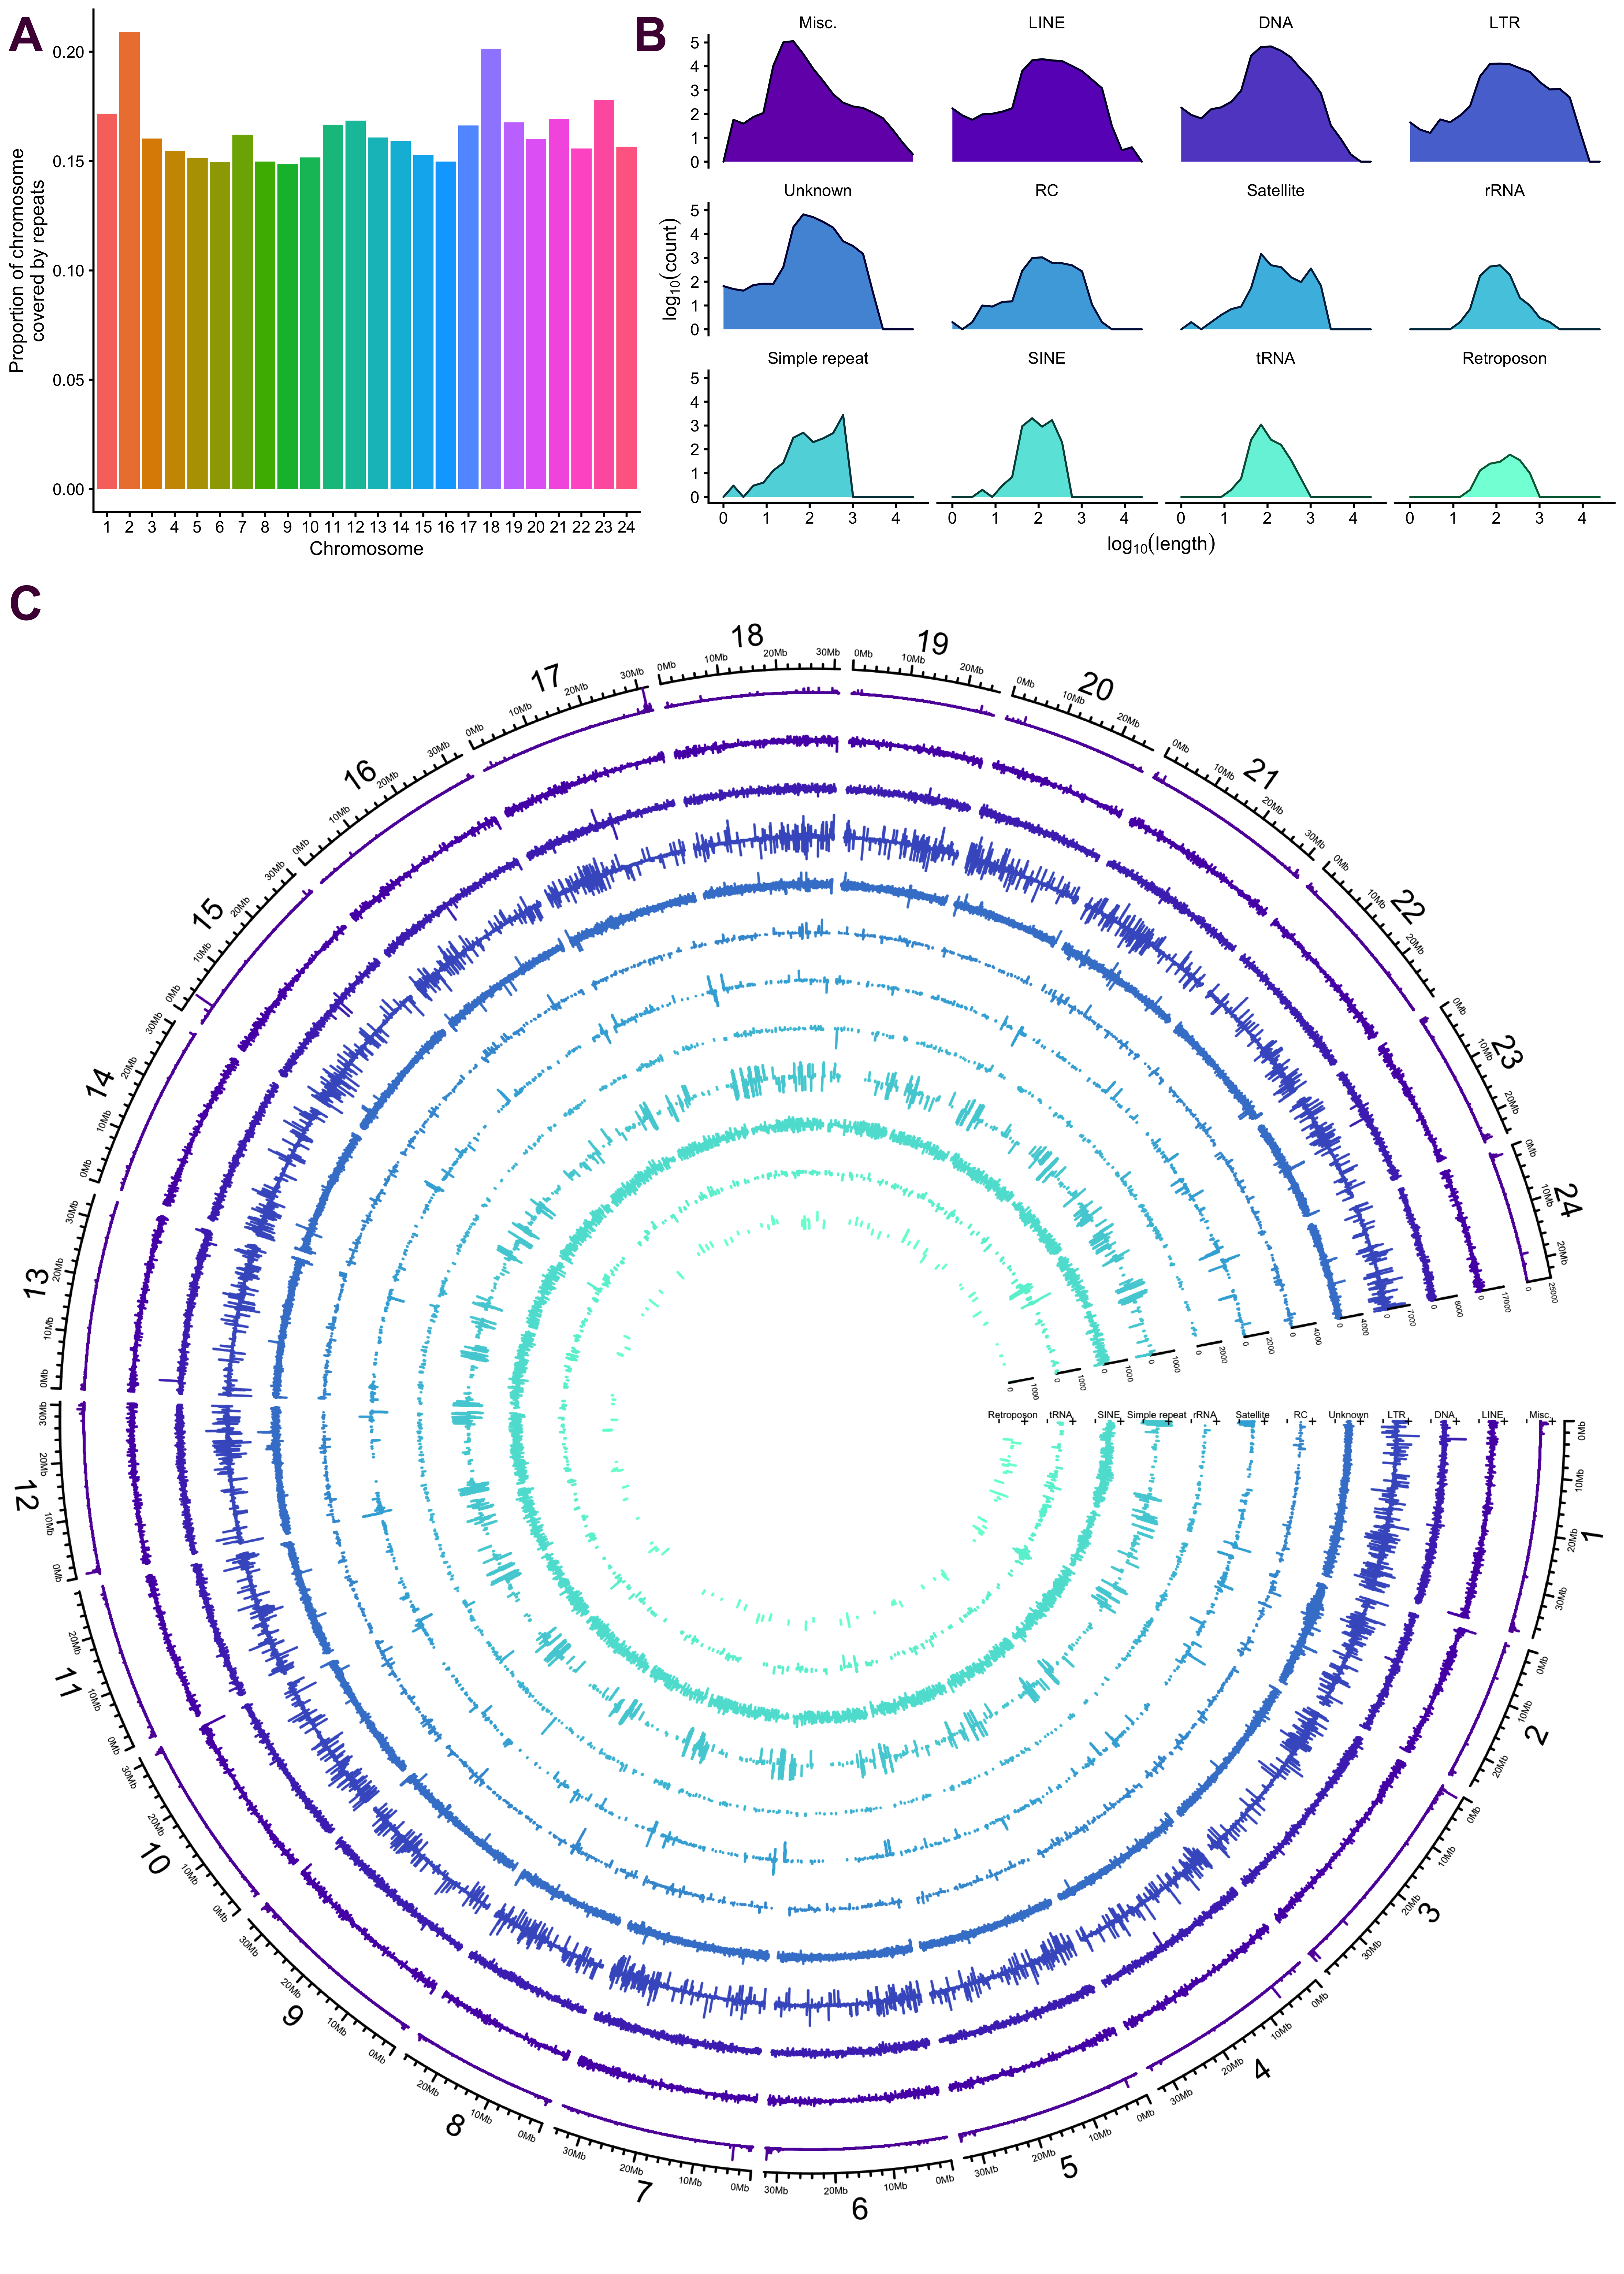
\includegraphics[width=1\linewidth]{figs/mikk_genome/20210401_hdrr_repeats_final} \caption{Repeat content in the \emph{HdrR} genome based on RepeatMasker results obtained by Jack Monahan. \textbf{A}. Proportion of repeat content per-chromosome. \textbf{B}. log10 of repeat lengths and counts per repeat class. ``Misc'' includes all repeats assigned to their own specific class, for example ``(GAG)n'' or ``(GATCCA)n''. \textbf{C}. Circos plot showing repeat length (radial axes) by locus (angular axis) and repeat class (track).}\label{fig:repeats}
\end{figure}

\hypertarget{mikksv-sec}{%
\section{Structural variation in the MIKK panel}\label{mikksv-sec}}

As an alternative to the variation pangenome approach described in Leger et al.\footnote{{``Genomic Variations and Epigenomic Landscape of the {Medaka Inbred Kiyosu-Karlsruhe} ({MIKK}) Panel.''}}, I explored the structural variants (SVs) present in 9 of the MIKK panel lines in a reference-anchored manner, similar to many human studies. Differences in SVs between panel lines is another important class of genetic variation that could cause or contribute to significant phenotypic differences. Here we used ONT data obtained for 9 of the 12 selected lines allowing us to characterise larger SVs in the MIKK panel and to create a more extensive picture of genomic rearrangements compared to available medaka reference genomes. Adrien Leger from the Birney Group at EMBL-EBI first called structural variants using only the ONT long reads, producing a set of structural variants classified into five types: deletions (DEL), insertions (INS), translocations (TRA), duplications (DUP) and inversions (INV). I then ``polished'' the called DEL and INS variants with Illumina short reads to improve their accuracy. The polishing process filtered out 7.4\% of DEL and 12.8\% of INS variants, and adjusted the breakpoints (i.e.~start and end positions) for 75-77\% of DEL and INS variants in each sample by a mean of 23 bp for the start position, and 33 bp for the end position. This process produced a total of 143,326 filtered SVs.

The 9 ``polished'' samples contained a mean per-sample count of approximately 37K DEL variants (12\% singletons), 29.5K INS variants (14\%), 3.5K TRA variants (9\%), 2.5K DUP (7\%) and 600 INV (7\%) (\textbf{Fig. \ref{fig:SV-main}D}). DEL variants were up to 494 kb in length, with 90\% of unique DEL variants shorter than 3.8 kb. INS variants were only up to 13.8 kb in length, with 90\% of unique INS variants shorter than 2 kb. DUP and INV variants tended to be longer, with a mean length of 19 and 70.5 kb respectively (\textbf{Fig. \ref{fig:SV-main}A}). \textbf{Fig. \ref{fig:SV-main}E} shows the per-sample distribution of DEL variants across the genome. Most large DEL variants over 250 kb in length were common among the MIKK panel lines. A number of large DEL variants appear to have accumulated within the 0-10 Mb region of chromosome 2, which is enriched for repeats in the HdrR reference genome (\textbf{Fig. \ref{fig:repeats}}).

SVs were generally enriched in regions covered by repeats. While only 16\% of bases in the \emph{HdrR} reference were classified as repeats (irrespective of strand), those bases overlapped with 72\% of DEL, 63\% of DUP, 81\% of INV and 35\% of TRA variant regions. However, repeat bases only overlapped with 21\% of INS variants. We also assessed each SV's probability of being loss-of-function (pLI)\footnote{Monkol Lek et al., {``Analysis of Protein-Coding Genetic Variation in 60,706 Humans,''} \emph{Nature} 536, no. 7616, 7616 (August 2016): 285--91, \url{https://doi.org/10.1038/nature19057}.} by calculating the logarithm of odds (LOD) for the pLI scores of all genes overlapping the variant (\textbf{Fig. \ref{fig:SV-main}B,C}). 30,357 out of 134,088 DEL, INS, DUP and INV variants overlapped at least one gene, and 9\% of those had a score greater than 10, indicating a high probability that the SV would cause a loss of function. Two INS variants on chr2 had an outlying LOD score of 57 as a result of overlapping medaka gene ENSORLG00000003411, which has a pLI score of 1 -- the highest intolerance to variants causing a loss of function. This gene is homologous with human genes \emph{SCN1A}, \emph{SCN2A} and \emph{SCN3A}, which encode sodium channels and have been associated with neuronal and sleep disorders. We did not find evidence that longer SVs tended to have a higher probability of causing a loss of function (\textbf{Fig. \ref{fig:SV-main}B}).



\begin{figure}
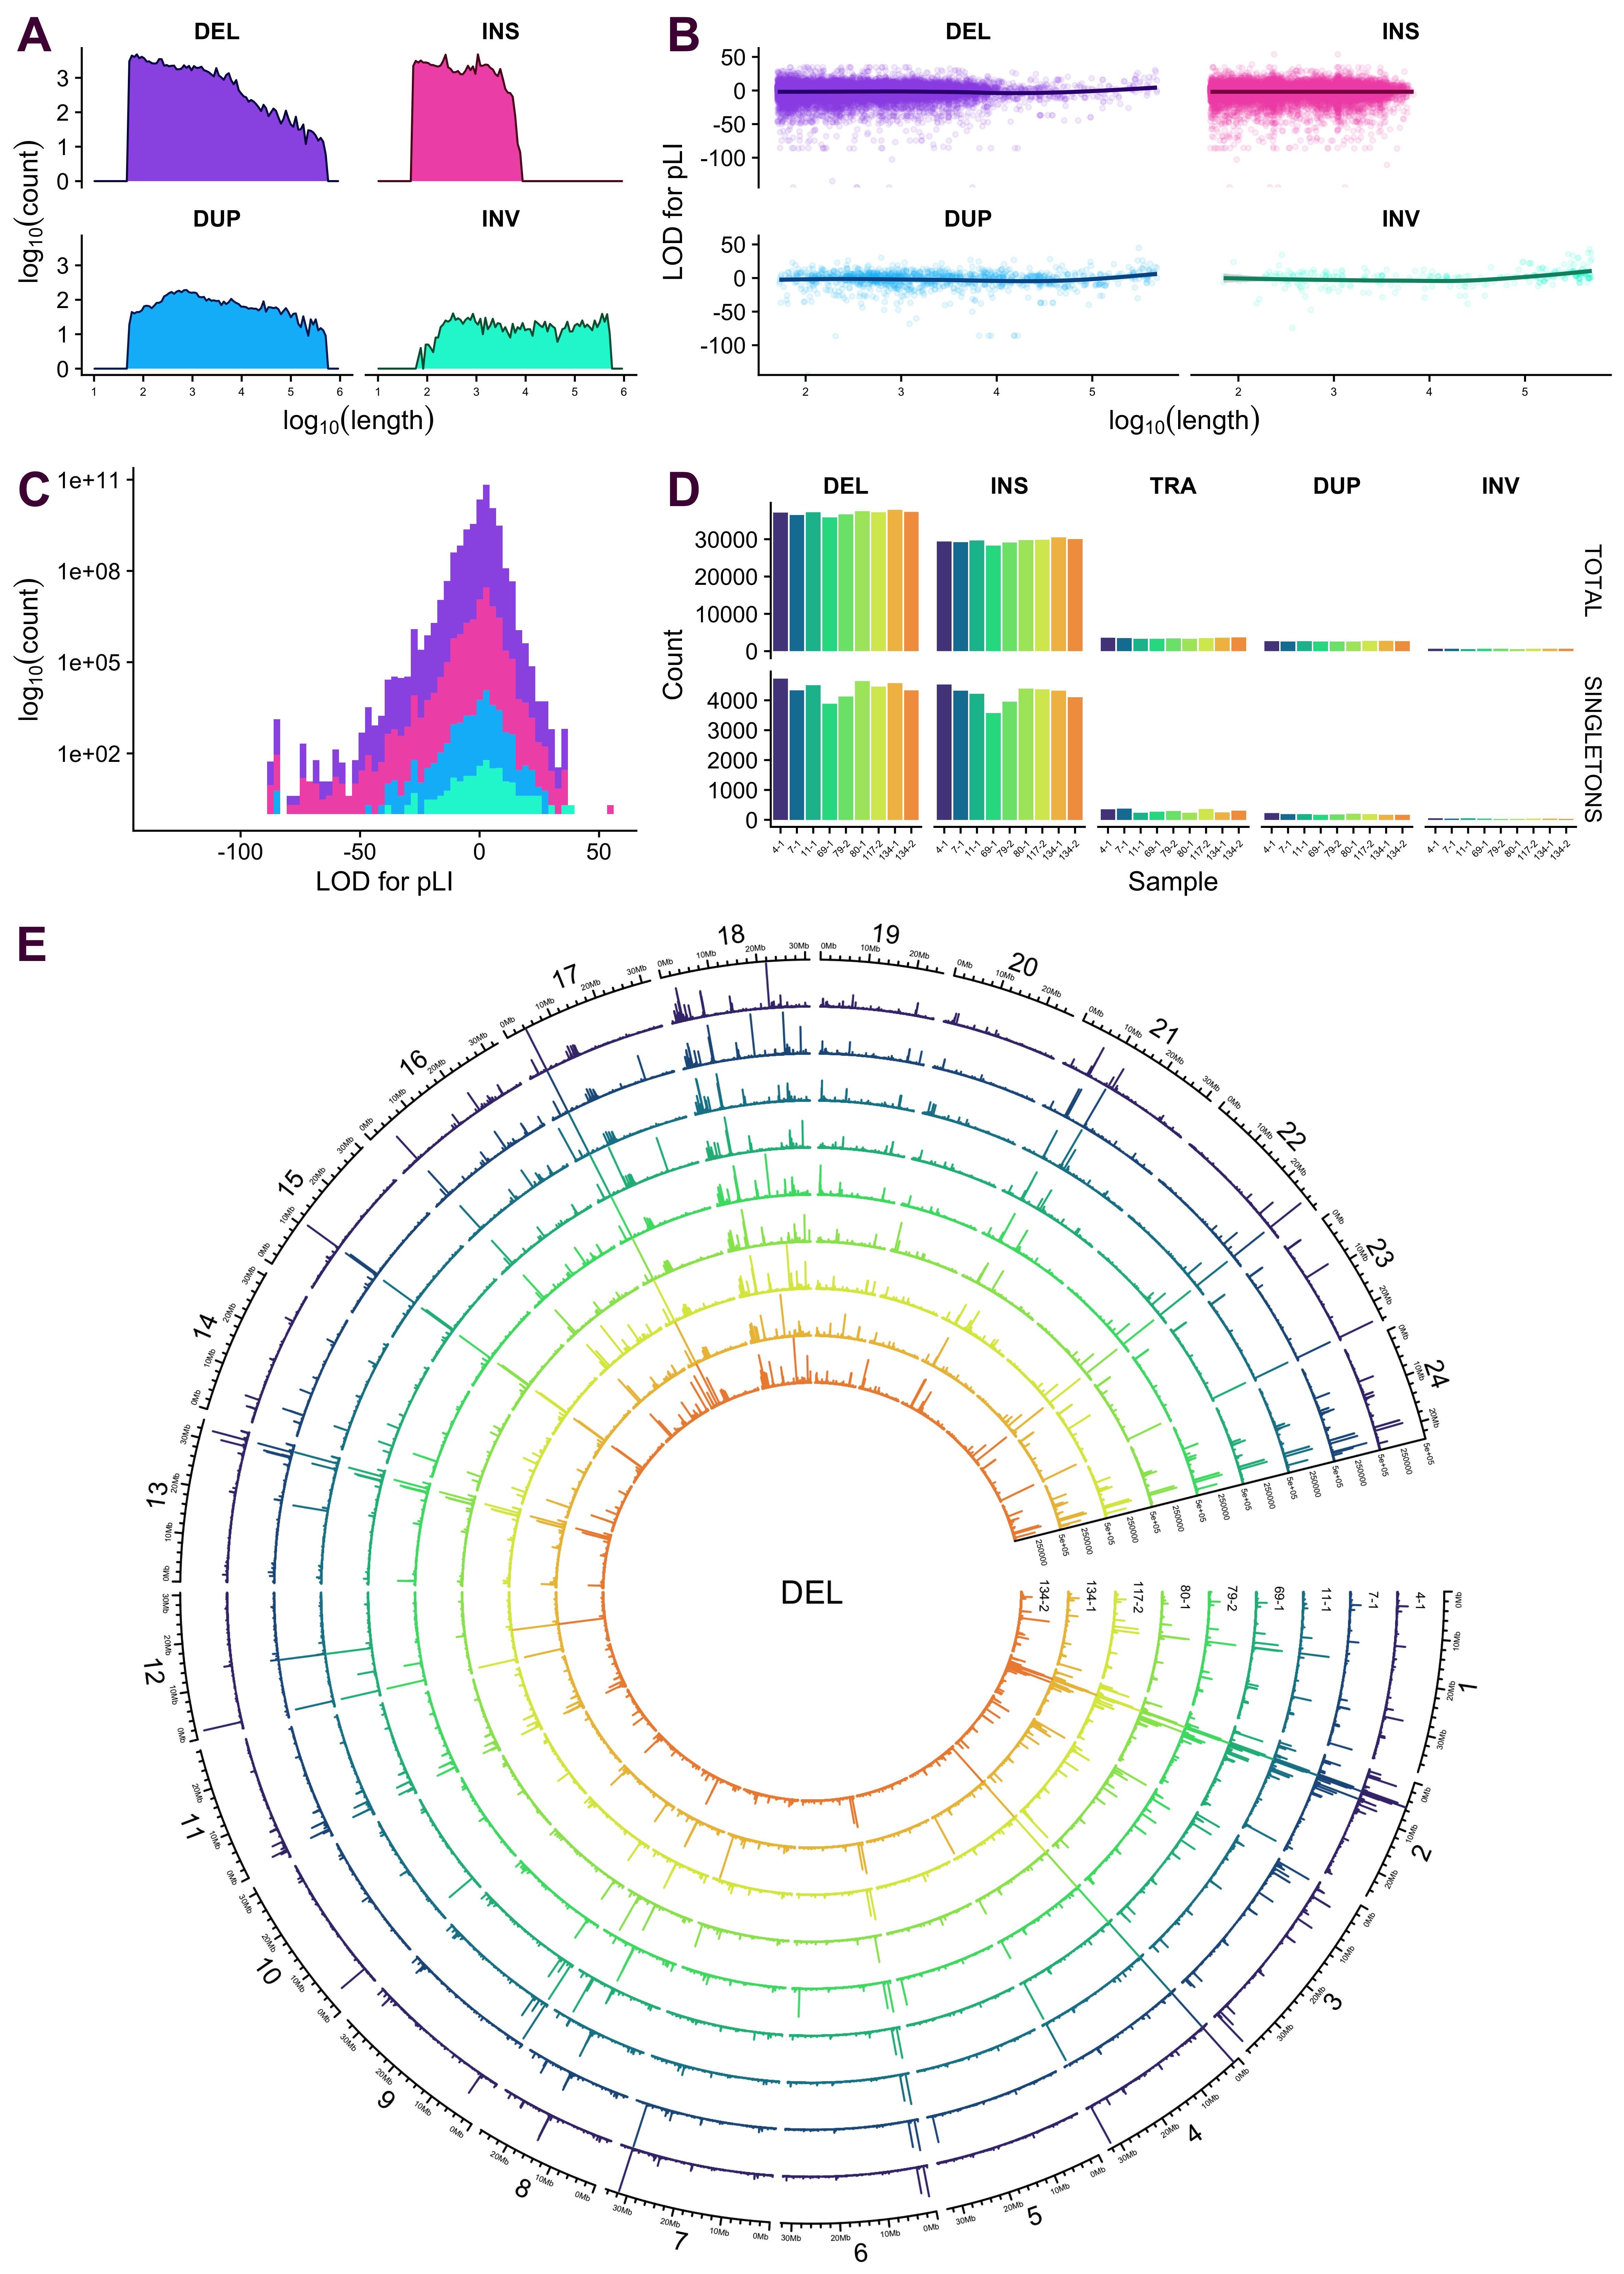
\includegraphics[width=1\linewidth]{figs/mikk_genome/20210408_sv_main} \caption{Polished SVs in 9 MIKK panel lines sequenced with ONT. DEL: deletion; INS: insertion; TRA: translocation; DUP: duplication; INV: inversion. \textbf{A}. Aggregate log10 counts and lengths of distinct SVs by type, excluding TRA. \textbf{B}. pLI LOD scores in distinct SVs by SV type. \textbf{C}. Histogram of LOD scores by SV type. \textbf{D}. Total and singleton counts of SV types per sample. \textbf{E}. Circos plot showing per-sample distribution and lengths of DEL variants across the genome.}\label{fig:SV-main}
\end{figure}

We compared these polished INS and DEL calls with the high-quality graph-based alternative paths and large-scale deletions, respectively (see section titled \emph{Novel genetic sequences and large-scale insertions and deletions in the MIKK panel} in Leger et al.\footnote{{``Genomic Variations and Epigenomic Landscape of the {Medaka Inbred Kiyosu-Karlsruhe} ({MIKK}) Panel.''}}). We found that 2 of the 19 regions covered by graph-based alternative paths, and 4 of the 16 regions covered by graph-based deletions, had no SVs that overlapped those regions at all, which suggests they would have been missed entirely when using a reference-anchored approach alone.

With the exception of one alternative path on chromosome 20, the alternative paths were not captured by INS variants, which only covered up to 63\% of the bases in each region, and in many cases substantially less. On the other hand, for 8 of the 16 graph-based deletions, the DEL variants covered at least 85\% of the bases in those regions. The other 8 graph-based deletions were either not at all covered by DEL variants, or only slightly. This indicates that the reference-based approach is better at detecting large-scale deletions than alternative paths (``insertions''), but still misses around half of such variants relative to the graph-based approach.

\hypertarget{conclusions}{%
\section{Conclusions}\label{conclusions}}

Taken together, these analyses show that the MIKK panel is highly homozygous, with LD characteristics that will favour high-resolution genetic mapping relative to humans. In the future, the SV analysis performed on a subset of the MIKK panel will be expanded across the entire panel, which will permit the inclusion of both large- and small-scale variants in genetic linkage studies. I proceeded to use the MIKK panel to analyse bold/shy behaviours, as I describe in Chapter \ref{MIKK-F2-chap}, with a view to carrying out an F2-cross linkage study to identify genetic variants associated with differences in the behaviours of an individual, and the extent to which they transmit those behaviours to their social companions. However, before carrying out this study, we first ran a ``pilot'' study on 5 previously-established inbred lines to validate our behavioural assay. This is the subject of the following chapter.

\hypertarget{Pilot-chap}{%
\chapter{Classification of bold/shy behaviours in 5 inbred medaka lines}\label{Pilot-chap}}

\hypertarget{MIKK-F2-chap}{%
\chapter{Bold/shy behaviours in the MIKK panel}\label{MIKK-F2-chap}}

\hypertarget{Fst-chap}{%
\chapter{Variation in the frequency of trait-associated alleles across global human populations}\label{Fst-chap}}

\hypertarget{Fst-background}{%
\section{Background}\label{Fst-background}}

Humans have long sought to use genetic information to predict an individual's likely value for a given trait, in our own species and for other organisms (Chapter \ref{Introduction}). As seen in previous chapters, an individual's phenotypic value at a given point in time is the product of complex interactions between their genome and their environment, beginning from embryonic development and continuing throughout their lifetimes.

It is now clear that ``complex'' traits such as height, intelligence, and behaviour are highly polygenic, meaning that they are genetically influenced by hundreds or thousands of genetic variants, each exerting a small effect in one or the other direction along the trait's spectrum.\footnote{G. Sella and N. Barton, {``Thinking {About} the {Evolution} of {Complex Traits} in the {Era} of {Genome-Wide Association Studies}.''} \emph{Annual Review of Genomics and Human Genetics}, 2019, \url{https://doi.org/10.1146/annurev-genom-083115-022316}.}

A richer understanding of the cumulative effect of genetic variants on any trait allows for the prediction of the value that an individual is most likely to have for that trait. Of all human traits, diseases are particularly salient; in 2018, the global healthcare industry was valued at US\$8 trillion, and predicted to increase to US\$12 trillion by 2022.\footnote{{``The \$11.9 {Trillion Global Healthcare Market}: {Key Opportunities} \& {Strategies} (2014-2022) - {ResearchAndMarkets}.com,''} June 25, 2019, \url{https://www.businesswire.com/news/home/20190625005862/en/The-11.9-Trillion-Global-Healthcare-Market-Key-Opportunities-Strategies-2014-2022---ResearchAndMarkets.com}.} This strong financial imperative complements the moral imperative to reduce suffering, together driving the question of how to use genetic information to improve human health.

Recent technological developments have made it possible to sequence human genomes at scale, and it is thought that by combining detailed genetic information with with other environmental and phenotypic information (such as lifestyle or clinical factors), clinicians could move towards the practice of ``precision medicine'', where interventions could be tailored to their patients' unique risk profiles.\footnote{Naomi R. Wray, Michael E. Goddard, and Peter M. Visscher, {``Prediction of Individual Genetic Risk to Disease from Genome-Wide Association Studies,''} \emph{Genome Research} 17, no. 10 (January 10, 2007): 1520--28, \url{https://doi.org/10.1101/gr.6665407}.} The use of genetic information to predict individuals' values for a trait of interest entails the construction of metrics known as ``polygenic scores'' (\textbf{PGS}). When the trait is a disease, PGS is commonly known as polygenic risk scores (\textbf{PRS}), or genetic risk profiling, but I will use the term PGS to encompass both disease and non-disease traits.

\hypertarget{polygenic-scores-pgs-and-genome-wide-association-studies-gwas}{%
\subsection{Polygenic Scores (PGS) and Genome-Wide Association Studies (GWAS)}\label{polygenic-scores-pgs-and-genome-wide-association-studies-gwas}}

\hypertarget{pgs}{%
\subsubsection{PGS}\label{pgs}}

PGS using genetic information alone show modest yet reliable accuracy for the prediction of complex traits:\footnote{Alicia R. Martin, Masahiro Kanai, et al., {``Clinical Use of Current Polygenic Risk Scores May Exacerbate Health Disparities,''} \emph{Nature Genetics} 51, no. 4, 4 (April 2019): 584--91, \url{https://doi.org/10.1038/s41588-019-0379-x}.} the correlations between PGS and the trait value as measured by \(R^2\) have reached 0.24 for height,\footnote{Loic Yengo et al., {``Meta-Analysis of Genome-Wide Association Studies for Height and Body Mass Index in ∼700000 Individuals of {European} Ancestry,''} \emph{Human Molecular Genetics} 27, no. 20 (October 15, 2018): 3641--49, \url{https://doi.org/10.1093/hmg/ddy271}.} and 0.12-0.16 for educational attainment.\footnote{Aysu Okbay et al., {``Polygenic Prediction of Educational Attainment Within and Between Families from Genome-Wide Association Analyses in 3 Million Individuals,''} \emph{Nature Genetics}, March 31, 2022, 1--13, \url{https://doi.org/10.1038/s41588-022-01016-z}.} For a variety of health-related traits, PGS improve predictions beyond non-genetic clinical models -- these traits include blood pressure, breast cancer,\footnote{Paige Maas et al., {``Breast {Cancer Risk From Modifiable} and {Nonmodifiable Risk Factors Among White Women} in the {United States},''} \emph{JAMA Oncology} 2, no. 10 (October 1, 2016): 1295--1302, \url{https://doi.org/10.1001/jamaoncol.2016.1025}.} prostate cancer,,\footnote{Fredrick R. Schumacher et al., {``Association Analyses of More Than 140,000 Men Identify 63 New Prostate Cancer Susceptibility Loci,''} \emph{Nature Genetics} 50, no. 7, 7 (July 2018): 928--36, \url{https://doi.org/10.1038/s41588-018-0142-8}.} and type I diabetes.\footnote{Seth A. Sharp et al., {``Development and {Standardization} of an {Improved Type} 1 {Diabetes Genetic Risk Score} for {Use} in {Newborn Screening} and {Incident Diagnosis},''} \emph{Diabetes Care} 42, no. 2 (January 11, 2019): 200--207, \url{https://doi.org/10.2337/dc18-1785}.}

PGS scores can further be combined with lifestyle and clinical factors to improve the accuracy of predictions for diseases such as cardiovascular disease.\footnote{Amit V. Khera et al., {``Genome-Wide Polygenic Scores for Common Diseases Identify Individuals with Risk Equivalent to Monogenic Mutations,''} \emph{Nature Genetics} 50, no. 9, 9 (September 2018): 1219--24, \url{https://doi.org/10.1038/s41588-018-0183-z}; Iftikhar J. Kullo et al., {``Incorporating a {Genetic Risk Score Into Coronary Heart Disease Risk Estimates},''} \emph{Circulation} 133, no. 12 (March 22, 2016): 1181--88, \url{https://doi.org/10.1161/CIRCULATIONAHA.115.020109}; Pradeep Natarajan et al., {``Polygenic {Risk Score Identifies Subgroup With Higher Burden} of {Atherosclerosis} and {Greater Relative Benefit From Statin Therapy} in the {Primary Prevention Setting},''} \emph{Circulation} 135, no. 22 (May 30, 2017): 2091--101, \url{https://doi.org/10.1161/CIRCULATIONAHA.116.024436}; Martine Paquette et al., {``Polygenic Risk Score Predicts Prevalence of Cardiovascular Disease in Patients with Familial Hypercholesterolemia,''} \emph{Journal of Clinical Lipidology} 11, no. 3 (May 1, 2017): 725--732.e5, \url{https://doi.org/10.1016/j.jacl.2017.03.019}; Emmi Tikkanen et al., {``Genetic {Risk Prediction} and a 2-{Stage Risk Screening Strategy} for {Coronary Heart Disease},''} \emph{Arteriosclerosis, Thrombosis, and Vascular Biology} 33, no. 9 (September 2013): 2261--66, \url{https://doi.org/10.1161/ATVBAHA.112.301120}.}

Beyond trait prediction, PGS have also been harnessed by evolutionary biologists to test whether a set of causal variants are evolving across populations or over time. Jeremy J Berg et al.\footnote{{``Reduced Signal for Polygenic Adaptation of Height in {UK Biobank},''} ed. Magnus Nordborg et al., \emph{eLife} 8 (March 21, 2019): e39725, \url{https://doi.org/10.7554/eLife.39725}.} and Michael D Edge and Graham Coop\footnote{{``Reconstructing the {History} of {Polygenic Scores Using Coalescent Trees},''} \emph{Genetics} 211, no. 1 (January 1, 2019): 235--62, \url{https://doi.org/10.1534/genetics.118.301687}.} found that this tends to occur through small, coordinated shifts in their allele frequencies.

\hypertarget{gwas}{%
\subsubsection{GWAS}\label{gwas}}

PGS are calculated for an individual by summing trait-associated alleles identified by genome-wide association studies (\textbf{GWAS}), as weighted by the alleles' effect sizes.\footnote{L. Duncan et al., {``Analysis of Polygenic Risk Score Usage and Performance in Diverse Human Populations,''} \emph{Nature Communications} 10, no. 1, 1 (July 25, 2019): 3328, \url{https://doi.org/10.1038/s41467-019-11112-0}.} GWAS aim to identify genetic variants associated with traits by comparing the allele frequencies of individuals who share similar ancestries, but differ in the trait in question.\footnote{Emil Uffelmann et al., {``Genome-Wide Association Studies,''} \emph{Nature Reviews Methods Primers} 1, no. 1, 1 (August 26, 2021): 1--21, \url{https://doi.org/10.1038/s43586-021-00056-9}.} As of 2021, over 5,700 GWAS have been performed for more than 3,330 traits.\footnote{Uffelmann et al.}

However, most GWAS have been performed with individuals of European ancestry, despite only constituting 16\% of the present global population. Although the proportion of participants in GWAS from a non-European background increased from 4\% in 2009 to 16 \% in 2016),\footnote{Alice B. Popejoy and Stephanie M. Fullerton, {``Genomics Is Failing on Diversity,''} \emph{Nature} 538, no. 7624, 7624 (October 2016): 161--64, \url{https://doi.org/10.1038/538161a}.} as of 2019, 79\% of all GWAS participants recorded in the GWAS Catalog were of European ancestry, and the proportion of non-European individuals has remained the same or reduced since late 2014.\footnote{Martin, Kanai, et al., {``Clinical Use of Current Polygenic Risk Scores May Exacerbate Health Disparities.''}} This bias extends to PGS studies, where as of 2019, only 67\% of them included only participants of European ancestry, with another 19\% including only East Asian ancestry participants, and only 3.8\% with cohorts of African, Hispanic, or Indigenous ancestry.\footnote{Duncan et al., {``Analysis of Polygenic Risk Score Usage and Performance in Diverse Human Populations.''}}

It is therefore unsurprising that PGS scores are far better at predicting disease risk in individuals of European ancestry than in those of non-European ancestry.\footnote{Alicia R Martin, Christopher R Gignoux, et al., {``Human Demographic History Impacts Genetic Risk Prediction Across Diverse Populations,''} \emph{The American Journal of Human Genetics} 100, no. 4 (2017): 635--49, \url{https://doi.org/10.1016/j.ajhg.2017.03.004}; Martin, Kanai, et al., {``Clinical Use of Current Polygenic Risk Scores May Exacerbate Health Disparities.''}} For example, Martin, Gignoux, et al.\footnote{{``Human Demographic History Impacts Genetic Risk Prediction Across Diverse Populations.''}} found that height was predicted to decrease with genetic distance from Europeans, despite robust evidence that West Africans are as tall as Europeans on average. Indeed, the predictive accuracy of PGS scores decays with genetic divergence of the GWAS ``independent'' or ``test'' sample from the ``discovery'' or ``training'' sample, as established in both humans,\footnote{Martin, Gignoux, et al.; Martin, Kanai, et al., {``Clinical Use of Current Polygenic Risk Scores May Exacerbate Health Disparities.''}} and livestock.\footnote{Samuel A. Clark et al., {``The Importance of Information on Relatives for the Prediction of Genomic Breeding Values and the Implications for the Makeup of Reference Data Sets in Livestock Breeding Schemes,''} \emph{Genetics Selection Evolution} 44, no. 1 (February 9, 2012): 4, \url{https://doi.org/10.1186/1297-9686-44-4}; David Habier et al., {``The Impact of Genetic Relationship Information on Genomic Breeding Values in {German Holstein} Cattle,''} \emph{Genetics Selection Evolution} 42, no. 1 (February 19, 2010): 5, \url{https://doi.org/10.1186/1297-9686-42-5}; M. Pszczola et al., {``Reliability of Direct Genomic Values for Animals with Different Relationships Within and to the Reference Population,''} \emph{Journal of Dairy Science} 95, no. 1 (January 1, 2012): 389--400, \url{https://doi.org/10.3168/jds.2011-4338}.}

These differences in representation cause PGS scores to have a lower accuracy for individuals of non-European ancestry. For example, compared to PGS scores for those of European ancestry, PGS scores across multiple traits for individuals of African ancestry are \textasciitilde64-78\% less accurate,\footnote{Duncan et al., {``Analysis of Polygenic Risk Score Usage and Performance in Diverse Human Populations''}; Martin, Kanai, et al., {``Clinical Use of Current Polygenic Risk Scores May Exacerbate Health Disparities.''}} and for individuals of South-Asian ancestry \textasciitilde37\% less accurate, and \textasciitilde50\% less accurate for individuals of East-Asian ancestry.\footnote{Martin, Kanai, et al., {``Clinical Use of Current Polygenic Risk Scores May Exacerbate Health Disparities.''}}

\hypertarget{contributors-to-pgs-non-transferability}{%
\subsection{Contributors to PGS non-transferability}\label{contributors-to-pgs-non-transferability}}

What explains this disparity in predictive value? A number of factors may be responsible, including:

\begin{enumerate}
\def\labelenumi{\arabic{enumi}.}
\item
  The failure of GWAS to identify causal variants that either do not exist or are not identifiable within the ``discovery'' sample.\footnote{Martin, Kanai, et al.}
\item
  The sample populations may differ in linkage disequilibrium (\textbf{LD}) -- the correlation structure of the genome -- which would change the estimated effect sizes of the causal variants, even when the causal variants themselves are the same.\footnote{Martin, Kanai, et al.}
\item
  Allele frequencies of the causal variants, and the distribution of the effect sizes of the causal variants, may differ between populations.\footnote{Martin, Gignoux, et al., {``Human Demographic History Impacts Genetic Risk Prediction Across Diverse Populations''}; Marco Scutari, Ian Mackay, and David Balding, {``Using {Genetic Distance} to {Infer} the {Accuracy} of {Genomic Prediction},''} \emph{PLOS Genetics} 12, no. 9 (September 2, 2016): e1006288, \url{https://doi.org/10.1371/journal.pgen.1006288}.}
\item
  The environments and demographies may differ between populations. These differences are often correlated with genetic divergence due to geography, making it difficult to determine whether the associations are driven by the differences between population in their genetics, or their environments.\footnote{Martin, Kanai, et al., {``Clinical Use of Current Polygenic Risk Scores May Exacerbate Health Disparities''}; Sini Kerminen et al., {``Geographic {Variation} and {Bias} in the {Polygenic Scores} of {Complex Diseases} and {Traits} in {Finland},''} \emph{The American Journal of Human Genetics} 104, no. 6 (June 6, 2019): 1169--81, \url{https://doi.org/10.1016/j.ajhg.2019.05.001}.}
\end{enumerate}

The first three factors can degrade predictive performance even in the absence of biological and environmental differences. On the other hand, environmental and demographic differences can drive forces of natural selection can in turn drive differences in causal genetic architecture.\footnote{Martin, Kanai, et al., {``Clinical Use of Current Polygenic Risk Scores May Exacerbate Health Disparities.''}}

Differences in LD and allele frequencies between populations can explain 70-80\% of the loss of PGS relative accuracy for traits like body mass index and type 2 diabetes.\footnote{Ying Wang et al., {``Theoretical and Empirical Quantification of the Accuracy of Polygenic Scores in Ancestry Divergent Populations,''} \emph{Nature Communications} 11, no. 1, 1 (July 31, 2020): 3865, \url{https://doi.org/10.1038/s41467-020-17719-y}.}

I discuss each of these factors in turn

\hypertarget{fst-discovery-sec}{%
\subsubsection{Failure to discover causal variants}\label{fst-discovery-sec}}

The power to discover a causal variant through GWAS depends on the variant's effect size and frequency in the study population.\footnote{Martin, Kanai, et al., {``Clinical Use of Current Polygenic Risk Scores May Exacerbate Health Disparities''}; P. C. Sham et al., {``Power of {Linkage} Versus {Association Analysis} of {Quantitative Traits}, by {Use} of {Variance-Components Models}, for {Sibship Data},''} \emph{The American Journal of Human Genetics} 66, no. 5 (May 1, 2000): 1616--30, \url{https://doi.org/10.1086/302891}.} That is to say, the stronger the variant's effect, or the more common it is, the more likely it is to be discovered. Rare variants tend to have stronger effect sizes,\footnote{Kyoko Watanabe et al., {``A Global Overview of Pleiotropy and Genetic Architecture in Complex Traits,''} \emph{Nature Genetics} 51, no. 9, 9 (September 2019): 1339--48, \url{https://doi.org/10.1038/s41588-019-0481-0}.} likely due to purifying selection,\footnote{Ju-Hyun Park et al., {``Distribution of Allele Frequencies and Effect Sizes and Their Interrelationships for Common Genetic Susceptibility Variants,''} \emph{Proceedings of the National Academy of Sciences} 108, no. 44 (November 2011): 18026--31, \url{https://doi.org/10.1073/pnas.1114759108}.} and tend not to be shared across populations.\footnote{Simon Gravel et al., {``Demographic History and Rare Allele Sharing Among Human Populations,''} \emph{Proceedings of the National Academy of Sciences} 108, no. 29 (2011): 11983--88, \url{https://doi.org/10.1073/pnas.1019276108}; 1000 Genomes Project Consortium et al., {``A Global Reference for Human Genetic Variation,''} \emph{Nature} 526, no. 7571 (2015): 68.}

There are several issues that can affect the discoverability of causal variants through GWAS, including the technology used for genotyping, the selection of the cohort, and the necessary exclusion of genotypic outliers.

With respect to genotyping technologies, GWAS often use data from SNP microarrays. These do not sequence the whole genome, but rather a selection (from several hundred thousand to millions) of genetic markers intended to present common genomic variation,\footnote{Eleonora Porcu et al., {``Genotype {Imputation} in {Genome-Wide Association Studies},''} \emph{Current Protocols in Human Genetics} 78, no. 1 (2013): 1.25.1--14, \url{https://doi.org/10.1002/0471142905.hg0125s78}.} which accordingly tend to neglect rare genetic variants.\footnote{Uffelmann et al., {``Genome-Wide Association Studies.''}} To increase the density of genotypes, which would increase the likelihood of refining the association signal and identifying causal variants, researchers often ``impute'' variants that aren't sequenced directly.\footnote{Porcu et al., {``Genotype {Imputation} in {Genome-Wide Association Studies}.''}} The imputation process involves ``phasing'' the study genotypes onto the genotypes of a ``reference panel.''\footnote{Shane McCarthy et al., {``A Reference Panel of 64,976 Haplotypes for Genotype Imputation,''} \emph{Nature Genetics} 48, no. 10, 10 (October 2016): 1279--83, \url{https://doi.org/10.1038/ng.3643}.} However, if the reference panel does not sufficiently represent the populations in the study sample, they are likely to miss or incorrectly impute those genotypes.\footnote{Martin, Kanai, et al., {``Clinical Use of Current Polygenic Risk Scores May Exacerbate Health Disparities.''}} This is particularly problematic for African populations, which are far more genetically diverse than European populations,\footnote{Consortium et al., {``A Global Reference for Human Genetic Variation.''}} making it difficult to capture a sufficient range of variation.

The neglect of rare variants can be overcome by using next-generation sequencing technologies such as whole-genome sequencing (\textbf{WGS}) and whole-exome sequencing (\textbf{WES}); the former seeks to sequence the full genome, and the latter of only targets the coding regions of the genome. However, these methods are more expensive, although as their costs continue to decrease, their application in large-scale GWAS is likely to become more widespread. \textbf{\emph{Alignment issues}}

A second issue is the selection of GWAS cohorts, which can introduce selection and collider biases.\footnote{Uffelmann et al., {``Genome-Wide Association Studies.''}} For instance, the UK Biobank, which contains genetic and phenotypic data on 500,000 participants recruited between 2006 and 2010, tend to be older, female, healthier, and wealthier than non-participants.\footnote{Anna Fry et al., {``Comparison of {Sociodemographic} and {Health-Related Characteristics} of {UK Biobank Participants With Those} of the {General Population},''} \emph{American Journal of Epidemiology} 186, no. 9 (November 1, 2017): 1026--34, \url{https://doi.org/10.1093/aje/kwx246}.}

A third issue is the ``quality control'' step that is required during the GWAS process.\footnote{Uffelmann et al., {``Genome-Wide Association Studies.''}} To avoid confounding from population stratification, which can lead to overestimated heritability and biased PGS, GWAS cohorts are filtered to include only those with similar ancestries -- or relative genetic homogeneity -- by clustering individuals through principal component analysis (\textbf{PCA}) of their genotypes. I elaborate on the issue of population stratification in section \ref{fst-env-sec} below.

\hypertarget{differences-in-ld}{%
\subsubsection{Differences in LD}\label{differences-in-ld}}

Because GWAS SNP markers are often not the causal variants themselves, but merely in physical proximity to them, the estimated effect size of a SNP marker depends on the extent to which it is in LD with the causal variant.\footnote{Hakhamanesh Mostafavi et al., {``Variable Prediction Accuracy of Polygenic Scores Within an Ancestry Group,''} ed. Ruth Loos, Michael B Eisen, and Paul O'Reilly, \emph{eLife} 9 (January 30, 2020): e48376, \url{https://doi.org/10.7554/eLife.48376}; Jonathan K. Pritchard and Molly Przeworski, {``Linkage {Disequilibrium} in {Humans}: {Models} and {Data},''} \emph{The American Journal of Human Genetics} 69, no. 1 (July 1, 2001): 1--14, \url{https://doi.org/10.1086/321275}.} To illustrate the problem, if a SNP has an LD \(r^2\) with a causal variant of 0.8 in the discovery population and 0.6 in the target population, it would explain 25\% = (1 - 0.6/0.8) less trait variation in the target population, and would therefore be less predictive.\footnote{Wang et al., {``Theoretical and Empirical Quantification of the Accuracy of Polygenic Scores in Ancestry Divergent Populations.''}}

Differences in effect-size estimates may typically be small for most regions of the genome, but as PGS sum across these effects, they aggregate these population differences.\footnote{Martin, Kanai, et al., {``Clinical Use of Current Polygenic Risk Scores May Exacerbate Health Disparities.''}} Previous empirical and simulation studies have shown that accuracy of PGS scores decay with increased genetic differentiation (\(F_{ST}\)) and LD differences between populations.\footnote{Habier et al., {``The Impact of Genetic Relationship Information on Genomic Breeding Values in {German Holstein} Cattle''}; Pszczola et al., {``Reliability of Direct Genomic Values for Animals with Different Relationships Within and to the Reference Population''}; Scutari, Mackay, and Balding, {``Using {Genetic Distance} to {Infer} the {Accuracy} of {Genomic Prediction}''}; Wang et al., {``Theoretical and Empirical Quantification of the Accuracy of Polygenic Scores in Ancestry Divergent Populations.''}}

It was demonstrated in simulations that using LD information from an external reference panel as a prior to infer the posterior mean effect size of a genetic variant can improve PGS predictive accuracy.\footnote{Bjarni J Vilhjálmsson et al., {``Modeling Linkage Disequilibrium Increases Accuracy of Polygenic Risk Scores,''} \emph{The American Journal of Human Genetics} 97, no. 4 (2015): 576--92.}

Genetic divergence between populations can be measured by \(F_{ST}\), and the correlation between true and predicted phenotypic values decays approximately linearly with respect to \(F_{ST}\).\footnote{Scutari, Mackay, and Balding, {``Using {Genetic Distance} to {Infer} the {Accuracy} of {Genomic Prediction}.''}}

\hypertarget{differences-in-allele-frequencies}{%
\subsubsection{Differences in allele frequencies}\label{differences-in-allele-frequencies}}

Causal variants can differ in both frequency and effect size between different ancestry groups, e.g.~for lactase persistence, or skin pigmentation.\footnote{Kaustubh Adhikari et al., {``A {GWAS} in {Latin Americans} Highlights the Convergent Evolution of Lighter Skin Pigmentation in {Eurasia},''} \emph{Nature Communications} 10, no. 1, 1 (January 21, 2019): 358, \url{https://doi.org/10.1038/s41467-018-08147-0}.} If a causal allele is rare in the GWAS discovery population, even if it is discovered (see \ref{fst-discovery-sec}) it is likely to have noisy effect size estimates, and therefore likely to inaccurately estimate its effect size in a different population where it exists at a higher frequency.

Differences in allele frequencies between populations can arise through random genetic drift, or be driven by selective pressures towards the trait optima for a given environment.\footnote{Arbel Harpak and Molly Przeworski, {``The Evolution of Group Differences in Changing Environments,''} \emph{PLOS Biology} 19, no. 1 (January 25, 2021): e3001072, \url{https://doi.org/10.1371/journal.pbio.3001072}.}

Chapter \ref{Fst-chap} will explore the differences in allele frequencies across populations for all polygenic traits in the GWAS Catalog, and demonstrate that with few exceptions -- including skin pigmentation, and HIV viral load -- the differences in allele frequencies between populations tends to be small. And therefore, the

\hypertarget{fst-env-sec}{%
\subsubsection{Differences in environment}\label{fst-env-sec}}

Genes interact with the environment to create phenotypic values.\footnote{Plomin and Asbury, {``Nature and {Nurture}.''}} Yet when it comes to the differences in mean values between groups (i.e.~populations) for traits that carry social benefit -- such as intelligence -- there is ongoing debate about what proportion of the variance that we observe between populations is genetic.

\begin{itemize}
\item
  The second issue is the same as what often affects the interpretation of the slippery biological concept of heritability. ``Heritability'' in its genetic sense describes the proportion of variance in a trait that is attributable to genetic factors. Because it is a \emph{proportion} of variance, when studying a population that is subject to greater environmental variation, the variance attributable to genetic factors will proportionately reduce. Conversely, when studying a population where the environment is held constant, the heritability for that trait will approach 1. PGS also measure the proportion of variance within a population that is explained by genetics, and the higher that proportion, the more accurate the predictions will be. So in the same way as heritability, increases in the amount of environmental variance in a population will reduce the proportion of variance explained by genetics.
\item
  The third issue is the confounding that different environments often have with population structure.\footnote{Berg et al., {``Reduced Signal for Polygenic Adaptation of Height in {UK Biobank}.''}} For example, in East Asia, there is a greater proportion of individuals of East-Asian ancestry than there is of European ancestry, and \emph{vice versa} in Europe. Those East-Asian individuals will therefore tend to share more of their genetic background with each other than with Europeans, and that ``population structure'' will be correlated with the different environments that exist in East Asia compared to Europe. This makes it difficult to determine whether it is the environment or the population structure that is driving the differences between those populations.
\end{itemize}

\hypertarget{Fst-analysis-chap}{%
\section{Analysis}\label{Fst-analysis-chap}}

In this chapter I explore the distribution of \(F_{ST}\) scores for loci associated with 587 traits, a subset of the GWAS Catalog that passed our criteria for suitable polygenic traits (see Chapter \ref{Fst-analysis-chap}). Using high-coverage sequence data for 2,504 individuals from the 1000 Genomes Project phase 3 release, for each trait in the GWAS Catalog we calculated the distribution of \(F_{ST}\) across all approximately-unlinked SNPs associated with it (trait SNPs), and compared these \(F_{ST}\) distributions with the \(F_{ST}\) distributions of random-selected SNPs that were matched to the trait SNPs by their allele frequencies in European populations (control SNPs). Our results show that traits related to the physical correlates of ``race'' (such as skin-pigmentation, eye colour, and hair shape) tend to have relatively high \(F_{ST}\) values -- signifying relatively high variance in allele frequencies between populations -- whereas traits related to intelligence (such as self-reported EA, mathematical ability, and cognitive function measurement) tend to have lower \(F_{ST}\) values that are similar to those of most polygenic traits such as height and body mass index.

\hypertarget{datasets}{%
\subsection{Datasets}\label{datasets}}

\hypertarget{genomes}{%
\subsubsection{1000 Genomes}\label{genomes}}

As the reference for human genomic variation across diverse populations, we used the New York Genome Center high-coverage, phased .vcf files\footnote{{``Index of /Vol1/Ftp/Data\_collections/{1000g}\_2504\_high\_coverage/Working/20201028\_3202\_phased/,''} accessed March 24, 2022, \url{http://ftp.1000genomes.ebi.ac.uk/vol1/ftp/data_collections/1000G_2504_high_coverage/working/20201028_3202_phased/}.} for the 2,504 individuals described in the 1000 Genomes phase 3 release.\footnote{Consortium et al., {``A Global Reference for Human Genetic Variation.''}} We then annotated those .vcf files with human SNP IDs from dbSNP release 9606.\footnote{Elizabeth M. Smigielski et al., {``{dbSNP}: A Database of Single Nucleotide Polymorphisms,''} \emph{Nucleic Acids Research} 28, no. 1 (January 1, 2000): 352--55, \url{https://doi.org/10.1093/nar/28.1.352}.}

\hypertarget{gwas-catalog}{%
\subsubsection{GWAS Catalog}\label{gwas-catalog}}

We used the R package \emph{gwasrapidd}\footnote{Ramiro Magno and Ana-Teresa Maia, {``Gwasrapidd: An {R} Package to Query, Download and Wrangle {GWAS} Catalog Data,''} \emph{Bioinformatics} 36, no. 2 (January 15, 2020): 649--50, \url{https://doi.org/10.1093/bioinformatics/btz605}.} to query all traits in the GWAS Catalog\footnote{Jacqueline MacArthur et al., {``The New {NHGRI-EBI Catalog} of Published Genome-Wide Association Studies ({GWAS Catalog}),''} \emph{Nucleic Acids Research} 45, no. D1 (January 4, 2017): D896--901, \url{https://doi.org/10.1093/nar/gkw1133}.} as of 9 August 2021 (\(N_{TRAITS}\) = 3,459). For 541 of these traits, no matching variant IDs could be pulled out from the 1000 Genomes VCFs, leaving \(N_{TRAITS}\) = 3,008.

\hypertarget{linkage-disequilibrium}{%
\subsection{Linkage disequilibrium}\label{linkage-disequilibrium}}

To obtain the ``trait SNP'' dataset, for each trait, we sought to isolate the SNP closest to each of its true causal variants, and exclude the SNPs in linkage disequilibrium (LD) with them. To this end, we used PLINK 1.9\footnote{Chang et al., {``Second-Generation {PLINK}''}; Purcell and Chang, \emph{{PLINK} 1.9}.} to ``clump'' the SNPs associated with each of the remaining 3,008 traits, using an ``index'' SNP p-value threshold of \(10^{-8}\),\footnote{Orestis A. Panagiotou, John P. A. Ioannidis, and Genome-Wide Significance Project, {``What Should the Genome-Wide Significance Threshold Be? {Empirical} Replication of Borderline Genetic Associations,''} \emph{International Journal of Epidemiology} 41, no. 1 (February 2012): 273--86, \url{https://doi.org/10.1093/ije/dyr178}.} \(r^2\) threshold of 0.1,\footnote{W. G. Hill and Alan Robertson, {``Linkage Disequilibrium in Finite Populations,''} \emph{Theoretical and Applied Genetics} 38, no. 6 (June 1, 1968): 226--31, \url{https://doi.org/10.1007/BF01245622}.} and base window size of 1 Mb. This process left us with 2,045 traits with at least one index SNP that met the p-value threshold. The index SNPs for each trait formed our set of trait SNPs, and \textbf{Figure \ref{fig:FstSnpCount}} shows the counts of unique SNP IDs associated with each trait before and after clumping. In order to target relatively polygenic traits, we further filtered out traits with fewer than 10 trait SNPs, leaving \(N_{TRAITS}\) = 587.



\begin{figure}
\includegraphics[width=1\linewidth]{figs/fst/0.1_1000_20220314_snp_counts} \caption{log10 counts of associated SNPs for each trait before and after the clumping process, which involved: a) excluding all SNPs with a \emph{p}-value greater than \(10^{-8}\); and b) starting with the SNPs with the lowest \emph{p}-values (``index'' SNPs), excluding all other SNPs within a 1 Mb region of the index SNP with an LD \(r^2\) of more than 0.1.}\label{fig:FstSnpCount}
\end{figure}

\hypertarget{control-snps}{%
\subsection{Control SNPs}\label{control-snps}}

To obtain our ``control SNP'' dataset, we assigned each trait SNP to one of 20 bins based on its minor allele frequency in European populations (as provided in the original 1000 Genomes .vcf files under the column header `INFO/AC\_EUR'). For example, if a trait SNP had a minor allele frequency of 0.08 in European populations, it was assigned to the \((0.05, 0.1]\) bin. I did the same for all (un-associated) SNPs in the .vcf files, then paired each trait SNP with a random SNP from the .vcf file in the equivalent bin. These allele-frequency-paired random SNPs formed our set of ``control SNPs'', which I used to infer the \(F_{ST}\) distribution of a random set of SNPs with the same allele frequencies as the trait SNPs, and against which I could compare the \(F_{ST}\) distribution of the trait SNPs.

\hypertarget{f_st-and-ranking-traits-by-signed-kolmogorov-smirnov-d-statistic}{%
\subsection{\texorpdfstring{\(F_{ST}\) and ranking traits by signed Kolmogorov-Smirnov \(D\) statistic}{F\_\{ST\} and ranking traits by signed Kolmogorov-Smirnov D statistic}}\label{f_st-and-ranking-traits-by-signed-kolmogorov-smirnov-d-statistic}}

I then calculated \(F_{ST}\) for each of the trait SNPs and their matched control SNPs using the Weir and Cockerham method,\footnote{B. S. Weir and C. Clark Cockerham, {``Estimating {F-Statistics} for the {Analysis} of {Population Structure},''} \emph{Evolution} 38, no. 6 (1984): 1358--70, \url{https://doi.org/10.2307/2408641}.} as implemented in the R package \emph{pegas}.\footnote{Emmanuel Paradis, {``Pegas: An {R} Package for Population Genetics with an Integrated--Modular Approach,''} \emph{Bioinformatics} 26, no. 3 (February 1, 2010): 419--20, \url{https://doi.org/10.1093/bioinformatics/btp696}.} To rank all traits based on the directional difference in \(F_{ST}\) distributions between trait and control SNPs, I ran three Kolmogorov-Smirnov (KS) tests for each trait \(t\) with \(x_t\) = \(F_{ST, trait SNPs}\) and \(y_t\) = \(F_{ST, control SNPs}\):

\begin{enumerate}
\def\labelenumi{\arabic{enumi}.}
\item
  two-sided (\(D_t\)) ;
\item
  one-sided ``greater'' (\(D_t^+\)) ; and
\item
  one-sided ``less'' (\(D_t^-\)).
\end{enumerate}

I note that \(D_{t} = max(D_t^+, D_t^-)\), where \(D_t^+\) is the greatest vertical distance attained by the eCDF of \(x_t\) over the eCDF of \(y_t\), and \(D_t^-\) is the greatest vertical distance attained by the eCDF of \(y_t\) over the eCDF of \(x_t\).\footnote{W. J. Conover, \emph{Practical {Nonparametric Statistics}} ({John Wiley \& Sons}, 1999), \url{https://books.google.com?id=n_39DwAAQBAJ}; J. Durbin, \emph{Distribution {Theory} for {Tests Based} on {Sample Distribution Function}} ({SIAM}, 1973), \url{https://books.google.com?id=zAryCrT1IUYC}.} Accordingly, we used a comparison of \(D_t^+\) and \(D_t^-\) to formulate a signed D statistic (\(D_t^S\)), based on the logic that trait SNPs with a lower overall \(F_{ST}\) than control SNPs tend to have a higher \(D\) under the ``greater'' test than the ``less'' test, and vice versa.

Therefore, \({D_t^S}\):

\[
\begin{aligned}
D_t^- > D_t^+ &: &-D_t \\
D_t^- = D_t^+ &: &0 \\
D_t^- < D_t^+ &: &D_t \\
\end{aligned}
\]

In \textbf{Figure \ref{fig:FstMain}} I present the \(F_{ST}\) distributions of trait SNPs for an illustrative subset of 28 human traits, ranked by \({D_t^S}\) when compared with their matched control SNPs. \textbf{Figure \ref{fig:FstMain}A} shows the densities of SNPs as a function of \(F_{ST}\), and \textbf{Figure \ref{fig:FstMain}B and C} show their empirical Cumulative Distribution Functions (eCDFs). \textbf{Figure \ref{fig:FstMain}B} includes the eCDFs of control SNPs in grey. eCDF figures for all 587 traits that passed our filters (Methods) are provided in \ref{fig:eCDFall}.



\begin{figure}
\includegraphics[width=1\linewidth]{figs/fst/0.1_1000_20220314_final} \caption{Distributions of \(F_{ST}\) across 28 illustrative human traits, ranked by signed-D (Kolmogorov-Smirnov test) comparing trait and control SNPs. \textbf{A}. \(F_{ST}\) density ridge plots with SNP markers. \textbf{B}. Empirical Cumulative Distribution Functions (eCDFs) of \(F_{ST}\) for trait-associated (colour) and random control (grey) SNPs, faceted by trait. \textbf{C}. Consolidated eCDFs of trait-associated SNPs from (B). eCDFs for all traits are included in Supplementary Figure 1.}\label{fig:FstMain}
\end{figure}

\hypertarget{implications}{%
\section{Implications}\label{implications}}

The low \(F_{ST}\) that we see for trait-associated alleles across various polygenic traits show that their allele frequencies do not substantially differ between populations. This means that, generally speaking, the genetic architecture of polygenic traits is shared across global populations.

This leads to the conclusion that the poor transferability of PGS across populations is not primarily driven by differences in trait-associated allele frequencies, but must rather by caused by differences in LD structure and environment.

\hypertarget{f_st-has-no-connection-with-mean-population-values}{%
\subsection{\texorpdfstring{\(F_{ST}\) has no connection with mean population values}{F\_\{ST\} has no connection with mean population values}}\label{f_st-has-no-connection-with-mean-population-values}}

The loci of educational attainment have similar \(F_{ST}\) distributions to those of most polygenic traits.

As \(F_{ST}\) does not take into account the effect size or direction of the effect of the trait-associated allele, for highly-polygenic traits like the ones shown here, \(F_{ST}\) is almost entirely decoupled from the mean additive genetic value (or polygenic risk score) between populations.\footnote{Jeremy J. Berg and Graham Coop, {``A {Population Genetic Signal} of {Polygenic Adaptation},''} \emph{PLOS Genetics} 10, no. 8 (August 7, 2014): e1004412, \url{https://doi.org/10.1371/journal.pgen.1004412}.}

Height and BMI, which are under strong differential selection, look the same as other polygenic traits, which illustrates the limitations of this analysis {[}\textbf{CITE}{]}

\hypertarget{the-importance-of-environment-and-its-complex-interactions-with-genetics}{%
\subsection{The importance of environment, and its complex interactions with genetics}\label{the-importance-of-environment-and-its-complex-interactions-with-genetics}}

Genes interact with themselves (GxG, or ``epistasis''),\footnote{Pierre-Alexis Gros, Herv'e Le Nagard, and Olivier Tenaillon, {``The {Evolution} of {Epistasis} and {Its Links With Genetic Robustness}, {Complexity} and {Drift} in a {Phenotypic Model} of {Adaptation},''} \emph{Genetics} 182, no. 1 (May 1, 2009): 277--93, \url{https://doi.org/10.1534/genetics.108.099127}.} the genes of one's parents (``genetic nurture'', Augustine Kong et al.\footnote{{``The Nature of Nurture: {Effects} of Parental Genotypes,''} \emph{Science} 359, no. 6374 (January 26, 2018): 424--28, \url{https://doi.org/10.1126/science.aan6877}.}) or social companions (``social genetic effects'')\footnote{Benjamin W. Domingue et al., {``The Social Genome of Friends and Schoolmates in the {National Longitudinal Study} of {Adolescent} to {Adult Health},''} \emph{Proceedings of the National Academy of Sciences} 115, no. 4 (January 23, 2018): 702--7, \url{https://doi.org/10.1073/pnas.1711803115}; Amelie Baud et al., {``Genetic {Variation} in the {Social Environment Contributes} to {Health} and {Disease},''} \emph{PLOS Genetics} 13, no. 1 (January 25, 2017): e1006498, \url{https://doi.org/10.1371/journal.pgen.1006498}.} and Chapters \ref{Pilot-chap} and \ref{MIKK-F2-chap}, and the wider non-genetic environment (GxE).

\hypertarget{a-push-for-diversity-in-genetic-studies}{%
\subsection{A push for diversity in genetic studies}\label{a-push-for-diversity-in-genetic-studies}}

The obvious solution to this issue of non-transferability of PGS scores to diverse populations is to increase the representation of those populations in GWAS and PGS studies, as has been often proposed elsewhere.\footnote{Martin, Gignoux, et al., {``Human Demographic History Impacts Genetic Risk Prediction Across Diverse Populations''}; Alicia R Martin et al., {``The Critical Needs and Challenges for Genetic Architecture Studies in {Africa},''} \emph{Current Opinion in Genetics \& Development}, Genetics of {Human Origins}, 53 (December 1, 2018): 113--20, \url{https://doi.org/10.1016/j.gde.2018.08.005}; Stephanie A. Bien et al., {``The {Future} of {Genomic Studies Must Be Globally Representative}: {Perspectives} from {PAGE},''} \emph{Annual Review of Genomics and Human Genetics} 20, no. 1 (August 31, 2019): 181--200, \url{https://doi.org/10.1146/annurev-genom-091416-035517}; Martin, Kanai, et al., {``Clinical Use of Current Polygenic Risk Scores May Exacerbate Health Disparities''}; Giorgio Sirugo, Scott M. Williams, and Sarah A. Tishkoff, {``The {Missing Diversity} in {Human Genetic Studies},''} \emph{Cell} 177, no. 1 (March 21, 2019): 26--31, \url{https://doi.org/10.1016/j.cell.2019.02.048}; Genevieve L. Wojcik et al., {``Genetic Analyses of Diverse Populations Improves Discovery for Complex Traits,''} \emph{Nature} 570, no. 7762, 7762 (June 2019): 514--18, \url{https://doi.org/10.1038/s41586-019-1310-4}.}

\hypertarget{appendix}{%
\chapter*{Appendix}\label{appendix}}
\addcontentsline{toc}{chapter}{Appendix}

\hypertarget{ecdf-of-all-polygenic-traits-in-the-gwas-catalog-ranked-by-d_ts}{%
\section*{\texorpdfstring{eCDF of all polygenic traits in the GWAS Catalog ranked by \({D_t^S}\)}{eCDF of all polygenic traits in the GWAS Catalog ranked by \{D\_t\^{}S\}}}\label{ecdf-of-all-polygenic-traits-in-the-gwas-catalog-ranked-by-d_ts}}
\addcontentsline{toc}{section}{eCDF of all polygenic traits in the GWAS Catalog ranked by \({D_t^S}\)}



\begin{figure}
\includegraphics[width=1\linewidth]{figs/fst/0.1_1000_20220314_ecdf_all_faceted_with_controls_d_rank_long} \caption{587 traits from the GWAS Catalog that passed our filters for polygenic traits, ranked by \({D_t^S}\).}\label{fig:eCDFall}
\end{figure}

\hypertarget{references}{%
\chapter*{References}\label{references}}
\addcontentsline{toc}{chapter}{References}

\hypertarget{refs}{}
\begin{CSLReferences}{1}{0}
\leavevmode\vadjust pre{\hypertarget{ref-GlobalReferenceHuman2015}{}}%
{``A Global Reference for Human Genetic Variation.''} \emph{Nature} 526, no. 7571 (2015): 68--74. \url{https://doi.org/10.1038/nature15393}.

\leavevmode\vadjust pre{\hypertarget{ref-adhikariGWASLatinAmericans2019}{}}%
Adhikari, Kaustubh, Javier Mendoza-Revilla, Anood Sohail, Macarena Fuentes-Guajardo, Jodie Lampert, Juan Camilo Chac'on-Duque, Malena Hurtado, et al. {``A {GWAS} in {Latin Americans} Highlights the Convergent Evolution of Lighter Skin Pigmentation in {Eurasia}.''} \emph{Nature Communications} 10, no. 1, 1 (January 21, 2019): 358. \url{https://doi.org/10.1038/s41467-018-08147-0}.

\leavevmode\vadjust pre{\hypertarget{ref-baudGeneticVariationSocial2017}{}}%
Baud, Amelie, Megan K. Mulligan, Francesco Paolo Casale, Jesse F. Ingels, Casey J. Bohl, Jacques Callebert, Jean-Marie Launay, et al. {``Genetic {Variation} in the {Social Environment Contributes} to {Health} and {Disease}.''} \emph{PLOS Genetics} 13, no. 1 (January 25, 2017): e1006498. \url{https://doi.org/10.1371/journal.pgen.1006498}.

\leavevmode\vadjust pre{\hypertarget{ref-bergPopulationGeneticSignal2014a}{}}%
Berg, Jeremy J., and Graham Coop. {``A {Population Genetic Signal} of {Polygenic Adaptation}.''} \emph{PLOS Genetics} 10, no. 8 (August 7, 2014): e1004412. \url{https://doi.org/10.1371/journal.pgen.1004412}.

\leavevmode\vadjust pre{\hypertarget{ref-bergReducedSignalPolygenic2019}{}}%
Berg, Jeremy J, Arbel Harpak, Nasa Sinnott-Armstrong, Anja Moltke Joergensen, Hakhamanesh Mostafavi, Yair Field, Evan August Boyle, et al. {``Reduced Signal for Polygenic Adaptation of Height in {UK Biobank}.''} Edited by Magnus Nordborg, Mark I McCarthy, Magnus Nordborg, Nicholas H Barton, and Joachim Hermisson. \emph{eLife} 8 (March 21, 2019): e39725. \url{https://doi.org/10.7554/eLife.39725}.

\leavevmode\vadjust pre{\hypertarget{ref-bergelsonIdentifyingGenesUnderlying2010}{}}%
Bergelson, Joy, and Fabrice Roux. {``Towards Identifying Genes Underlying Ecologically Relevant Traits in {Arabidopsis} Thaliana.''} \emph{Nature Reviews Genetics} 11, no. 12, 12 (December 2010): 867--79. \url{https://doi.org/10.1038/nrg2896}.

\leavevmode\vadjust pre{\hypertarget{ref-bienFutureGenomicStudies2019}{}}%
Bien, Stephanie A., Genevieve L. Wojcik, Chani J. Hodonsky, Christopher R. Gignoux, Iona Cheng, Tara C. Matise, Ulrike Peters, Eimear E. Kenny, and Kari E. North. {``The {Future} of {Genomic Studies Must Be Globally Representative}: {Perspectives} from {PAGE}.''} \emph{Annual Review of Genomics and Human Genetics} 20, no. 1 (August 31, 2019): 181--200. \url{https://doi.org/10.1146/annurev-genom-091416-035517}.

\leavevmode\vadjust pre{\hypertarget{ref-changSecondgenerationPLINKRising2015}{}}%
Chang, Christopher C, Carson C Chow, Laurent CAM Tellier, Shashaank Vattikuti, Shaun M Purcell, and James J Lee. {``Second-Generation {PLINK}: Rising to the Challenge of Larger and Richer Datasets.''} \emph{GigaScience} 4, no. 1 (December 2015): 7. \url{https://doi.org/10.1186/s13742-015-0047-8}.

\leavevmode\vadjust pre{\hypertarget{ref-clarkImportanceInformationRelatives2012}{}}%
Clark, Samuel A., John M. Hickey, Hans D. Daetwyler, and Julius HJ van der Werf. {``The Importance of Information on Relatives for the Prediction of Genomic Breeding Values and the Implications for the Makeup of Reference Data Sets in Livestock Breeding Schemes.''} \emph{Genetics Selection Evolution} 44, no. 1 (February 9, 2012): 4. \url{https://doi.org/10.1186/1297-9686-44-4}.

\leavevmode\vadjust pre{\hypertarget{ref-conoverPracticalNonparametricStatistics1999}{}}%
Conover, W. J. \emph{Practical {Nonparametric Statistics}}. {John Wiley \& Sons}, 1999. \url{https://books.google.com?id=n_39DwAAQBAJ}.

\leavevmode\vadjust pre{\hypertarget{ref-10002015global}{}}%
Consortium, 1000 Genomes Project et al. {``A Global Reference for Human Genetic Variation.''} \emph{Nature} 526, no. 7571 (2015): 68.

\leavevmode\vadjust pre{\hypertarget{ref-domingueSocialGenomeFriends2018}{}}%
Domingue, Benjamin W., Daniel W. Belsky, Jason M. Fletcher, Dalton Conley, Jason D. Boardman, and Kathleen Mullan Harris. {``The Social Genome of Friends and Schoolmates in the {National Longitudinal Study} of {Adolescent} to {Adult Health}.''} \emph{Proceedings of the National Academy of Sciences} 115, no. 4 (January 23, 2018): 702--7. \url{https://doi.org/10.1073/pnas.1711803115}.

\leavevmode\vadjust pre{\hypertarget{ref-duncanAnalysisPolygenicRisk2019}{}}%
Duncan, L., H. Shen, B. Gelaye, J. Meijsen, K. Ressler, M. Feldman, R. Peterson, and B. Domingue. {``Analysis of Polygenic Risk Score Usage and Performance in Diverse Human Populations.''} \emph{Nature Communications} 10, no. 1, 1 (July 25, 2019): 3328. \url{https://doi.org/10.1038/s41467-019-11112-0}.

\leavevmode\vadjust pre{\hypertarget{ref-durbinDistributionTheoryTests1973}{}}%
Durbin, J. \emph{Distribution {Theory} for {Tests Based} on {Sample Distribution Function}}. {SIAM}, 1973. \url{https://books.google.com?id=zAryCrT1IUYC}.

\leavevmode\vadjust pre{\hypertarget{ref-edgeReconstructingHistoryPolygenic2019}{}}%
Edge, Michael D, and Graham Coop. {``Reconstructing the {History} of {Polygenic Scores Using Coalescent Trees}.''} \emph{Genetics} 211, no. 1 (January 1, 2019): 235--62. \url{https://doi.org/10.1534/genetics.118.301687}.

\leavevmode\vadjust pre{\hypertarget{ref-evansQTLGeneElegans2021}{}}%
Evans, Kathryn S., Marijke H. van Wijk, Patrick T. McGrath, Erik C. Andersen, and Mark G. Sterken. {``From {QTL} to Gene: {C}. Elegans Facilitates Discoveries of the Genetic Mechanisms Underlying Natural Variation.''} \emph{Trends in Genetics} 37, no. 10 (October 1, 2021): 933--47. \url{https://doi.org/10.1016/j.tig.2021.06.005}.

\leavevmode\vadjust pre{\hypertarget{ref-fitzgeraldMedakaInbredKiyosuKarlsruhe2022}{}}%
Fitzgerald, Tomas, Ian Brettell, Adrien Leger, Nadeshda Wolf, Natalja Kusminski, Jack Monahan, Carl Barton, et al. {``The {Medaka Inbred Kiyosu-Karlsruhe} ({MIKK}) Panel.''} \emph{Genome Biology} 23, no. 1 (February 21, 2022): 59. \url{https://doi.org/10.1186/s13059-022-02623-z}.

\leavevmode\vadjust pre{\hypertarget{ref-fredmanComplexSNPrelatedSequence2004}{}}%
Fredman, David, Stefan J. White, Susanna Potter, Evan E. Eichler, Johan T. Den Dunnen, and Anthony J. Brookes. {``Complex {SNP-related} Sequence Variation in Segmental Genome Duplications.''} \emph{Nature Genetics} 36, no. 8, 8 (August 2004): 861--66. \url{https://doi.org/10.1038/ng1401}.

\leavevmode\vadjust pre{\hypertarget{ref-fryComparisonSociodemographicHealthRelated2017}{}}%
Fry, Anna, Thomas J Littlejohns, Cathie Sudlow, Nicola Doherty, Ligia Adamska, Tim Sprosen, Rory Collins, and Naomi E Allen. {``Comparison of {Sociodemographic} and {Health-Related Characteristics} of {UK Biobank Participants With Those} of the {General Population}.''} \emph{American Journal of Epidemiology} 186, no. 9 (November 1, 2017): 1026--34. \url{https://doi.org/10.1093/aje/kwx246}.

\leavevmode\vadjust pre{\hypertarget{ref-gravel2011demographic}{}}%
Gravel, Simon, Brenna M Henn, Ryan N Gutenkunst, Amit R Indap, Gabor T Marth, Andrew G Clark, Fuli Yu, et al. {``Demographic History and Rare Allele Sharing Among Human Populations.''} \emph{Proceedings of the National Academy of Sciences} 108, no. 29 (2011): 11983--88. \url{https://doi.org/10.1073/pnas.1019276108}.

\leavevmode\vadjust pre{\hypertarget{ref-grosEvolutionEpistasisIts2009}{}}%
Gros, Pierre-Alexis, Herv'e Le Nagard, and Olivier Tenaillon. {``The {Evolution} of {Epistasis} and {Its Links With Genetic Robustness}, {Complexity} and {Drift} in a {Phenotypic Model} of {Adaptation}.''} \emph{Genetics} 182, no. 1 (May 1, 2009): 277--93. \url{https://doi.org/10.1534/genetics.108.099127}.

\leavevmode\vadjust pre{\hypertarget{ref-habierImpactGeneticRelationship2010}{}}%
Habier, David, Jens Tetens, Franz-Reinhold Seefried, Peter Lichtner, and Georg Thaller. {``The Impact of Genetic Relationship Information on Genomic Breeding Values in {German Holstein} Cattle.''} \emph{Genetics Selection Evolution} 42, no. 1 (February 19, 2010): 5. \url{https://doi.org/10.1186/1297-9686-42-5}.

\leavevmode\vadjust pre{\hypertarget{ref-harpakEvolutionGroupDifferences2021}{}}%
Harpak, Arbel, and Molly Przeworski. {``The Evolution of Group Differences in Changing Environments.''} \emph{PLOS Biology} 19, no. 1 (January 25, 2021): e3001072. \url{https://doi.org/10.1371/journal.pbio.3001072}.

\leavevmode\vadjust pre{\hypertarget{ref-hillLinkageDisequilibriumFinite1968}{}}%
Hill, W. G., and Alan Robertson. {``Linkage Disequilibrium in Finite Populations.''} \emph{Theoretical and Applied Genetics} 38, no. 6 (June 1, 1968): 226--31. \url{https://doi.org/10.1007/BF01245622}.

\leavevmode\vadjust pre{\hypertarget{ref-hoffmannChromosomalInversionPolymorphisms2004}{}}%
Hoffmann, Ary A., Carla M. Sgr`o, and Andrew R. Weeks. {``Chromosomal Inversion Polymorphisms and Adaptation.''} \emph{Trends in Ecology \& Evolution} 19, no. 9 (September 1, 2004): 482--88. \url{https://doi.org/10.1016/j.tree.2004.06.013}.

\leavevmode\vadjust pre{\hypertarget{ref-IndexPubRelease102}{}}%
{``Index of /Pub/Release-102/Emf/Ensembl-Compara/Multiple\_alignments/50\_fish.epo/.''} Accessed January 25, 2022. \url{https://ftp.ensembl.org/pub/release-102/emf/ensembl-compara/multiple_alignments/50_fish.epo/}.

\leavevmode\vadjust pre{\hypertarget{ref-IndexVol1Ftp}{}}%
{``Index of /Vol1/Ftp/Data\_collections/{1000g}\_2504\_high\_coverage/Working/20201028\_3202\_phased/.''} Accessed March 24, 2022. \url{http://ftp.1000genomes.ebi.ac.uk/vol1/ftp/data_collections/1000G_2504_high_coverage/working/20201028_3202_phased/}.

\leavevmode\vadjust pre{\hypertarget{ref-johnsonSegregationPerformanceRecombinant1999}{}}%
Johnson, William C., and Paul Gepts. {``Segregation for Performance in Recombinant Inbred Populations Resulting from Inter-Gene Pool Crosses of Common Bean ( {Phaseolus} Vulgaris {L}.).''} \emph{Euphytica} 106, no. 1 (March 1, 1999): 45--56. \url{https://doi.org/10.1023/A:1003541201923}.

\leavevmode\vadjust pre{\hypertarget{ref-katsumuraMedakaPopulationGenome2019}{}}%
Katsumura, Takafumi, Shoji Oda, Hiroshi Mitani, and Hiroki Oota. {``Medaka {Population Genome Structure} and {Demographic History Described} via {Genotyping-by-Sequencing}.''} \emph{G3 Genes\textbar Genomes\textbar Genetics} 9, no. 1 (January 1, 2019): 217--28. \url{https://doi.org/10.1534/g3.118.200779}.

\leavevmode\vadjust pre{\hypertarget{ref-kerminenGeographicVariationBias2019}{}}%
Kerminen, Sini, Alicia R. Martin, Jukka Koskela, Sanni E. Ruotsalainen, Aki S. Havulinna, Ida Surakka, Aarno Palotie, et al. {``Geographic {Variation} and {Bias} in the {Polygenic Scores} of {Complex Diseases} and {Traits} in {Finland}.''} \emph{The American Journal of Human Genetics} 104, no. 6 (June 6, 2019): 1169--81. \url{https://doi.org/10.1016/j.ajhg.2019.05.001}.

\leavevmode\vadjust pre{\hypertarget{ref-kheraGenomewidePolygenicScores2018}{}}%
Khera, Amit V., Mark Chaffin, Krishna G. Aragam, Mary E. Haas, Carolina Roselli, Seung Hoan Choi, Pradeep Natarajan, et al. {``Genome-Wide Polygenic Scores for Common Diseases Identify Individuals with Risk Equivalent to Monogenic Mutations.''} \emph{Nature Genetics} 50, no. 9, 9 (September 2018): 1219--24. \url{https://doi.org/10.1038/s41588-018-0183-z}.

\leavevmode\vadjust pre{\hypertarget{ref-kongNatureNurtureEffects2018}{}}%
Kong, Augustine, Gudmar Thorleifsson, Michael L. Frigge, Bjarni J. Vilhjalmsson, Alexander I. Young, Thorgeir E. Thorgeirsson, Stefania Benonisdottir, et al. {``The Nature of Nurture: {Effects} of Parental Genotypes.''} \emph{Science} 359, no. 6374 (January 26, 2018): 424--28. \url{https://doi.org/10.1126/science.aan6877}.

\leavevmode\vadjust pre{\hypertarget{ref-kulloIncorporatingGeneticRisk2016}{}}%
Kullo, Iftikhar J., Hayan Jouni, Erin E. Austin, Sherry-Ann Brown, Teresa M. Kruisselbrink, Iyad N. Isseh, Raad A. Haddad, et al. {``Incorporating a {Genetic Risk Score Into Coronary Heart Disease Risk Estimates}.''} \emph{Circulation} 133, no. 12 (March 22, 2016): 1181--88. \url{https://doi.org/10.1161/CIRCULATIONAHA.115.020109}.

\leavevmode\vadjust pre{\hypertarget{ref-legerGenomicVariationsEpigenomic2022}{}}%
Leger, Adrien, Ian Brettell, Jack Monahan, Carl Barton, Nadeshda Wolf, Natalja Kusminski, Cathrin Herder, et al. {``Genomic Variations and Epigenomic Landscape of the {Medaka Inbred Kiyosu-Karlsruhe} ({MIKK}) Panel.''} \emph{Genome Biology} 23, no. 1 (February 21, 2022): 58. \url{https://doi.org/10.1186/s13059-022-02602-4}.

\leavevmode\vadjust pre{\hypertarget{ref-lekAnalysisProteincodingGenetic2016}{}}%
Lek, Monkol, Konrad J. Karczewski, Eric V. Minikel, Kaitlin E. Samocha, Eric Banks, Timothy Fennell, Anne H. O'NADonnell-Luria, et al. {``Analysis of Protein-Coding Genetic Variation in 60,706 Humans.''} \emph{Nature} 536, no. 7616, 7616 (August 2016): 285--91. \url{https://doi.org/10.1038/nature19057}.

\leavevmode\vadjust pre{\hypertarget{ref-limamiGeneticPhysiologicalAnalysis2002}{}}%
Limami, Anis M., Clothilde Rouillon, Gaëlle Glevarec, Andr'e Gallais, and Bertrand Hirel. {``Genetic and {Physiological Analysis} of {Germination Efficiency} in {Maize} in {Relation} to {Nitrogen Metabolism Reveals} the {Importance} of {Cytosolic Glutamine Synthetase}.''} \emph{Plant Physiology} 130, no. 4 (December 1, 2002): 1860--70. \url{https://doi.org/10.1104/pp.009647}.

\leavevmode\vadjust pre{\hypertarget{ref-maasBreastCancerRisk2016}{}}%
Maas, Paige, Myrto Barrdahl, Amit D. Joshi, Paul L. Auer, Mia M. Gaudet, Roger L. Milne, Fredrick R. Schumacher, et al. {``Breast {Cancer Risk From Modifiable} and {Nonmodifiable Risk Factors Among White Women} in the {United States}.''} \emph{JAMA Oncology} 2, no. 10 (October 1, 2016): 1295--1302. \url{https://doi.org/10.1001/jamaoncol.2016.1025}.

\leavevmode\vadjust pre{\hypertarget{ref-macarthurNewNHGRIEBICatalog2017}{}}%
MacArthur, Jacqueline, Emily Bowler, Maria Cerezo, Laurent Gil, Peggy Hall, Emma Hastings, Heather Junkins, et al. {``The New {NHGRI-EBI Catalog} of Published Genome-Wide Association Studies ({GWAS Catalog}).''} \emph{Nucleic Acids Research} 45, no. D1 (January 4, 2017): D896--901. \url{https://doi.org/10.1093/nar/gkw1133}.

\leavevmode\vadjust pre{\hypertarget{ref-mackayChartingGenotypePhenotype2018}{}}%
Mackay, Trudy F. C., and Wen Huang. {``Charting the Genotype--Phenotype Map: Lessons from the {Drosophila} Melanogaster {Genetic Reference Panel}.''} \emph{WIREs Developmental Biology} 7, no. 1 (2018): e289. \url{https://doi.org/10.1002/wdev.289}.

\leavevmode\vadjust pre{\hypertarget{ref-magnoGwasrapiddPackageQuery2020}{}}%
Magno, Ramiro, and Ana-Teresa Maia. {``Gwasrapidd: An {R} Package to Query, Download and Wrangle {GWAS} Catalog Data.''} \emph{Bioinformatics} 36, no. 2 (January 15, 2020): 649--50. \url{https://doi.org/10.1093/bioinformatics/btz605}.

\leavevmode\vadjust pre{\hypertarget{ref-martinHumanDemographicHistory2017}{}}%
Martin, Alicia R, Christopher R Gignoux, Raymond K Walters, Genevieve L Wojcik, Benjamin M Neale, Simon Gravel, Mark J Daly, Carlos D Bustamante, and Eimear E Kenny. {``Human Demographic History Impacts Genetic Risk Prediction Across Diverse Populations.''} \emph{The American Journal of Human Genetics} 100, no. 4 (2017): 635--49. \url{https://doi.org/10.1016/j.ajhg.2017.03.004}.

\leavevmode\vadjust pre{\hypertarget{ref-martinClinicalUseCurrent2019}{}}%
Martin, Alicia R., Masahiro Kanai, Yoichiro Kamatani, Yukinori Okada, Benjamin M. Neale, and Mark J. Daly. {``Clinical Use of Current Polygenic Risk Scores May Exacerbate Health Disparities.''} \emph{Nature Genetics} 51, no. 4, 4 (April 2019): 584--91. \url{https://doi.org/10.1038/s41588-019-0379-x}.

\leavevmode\vadjust pre{\hypertarget{ref-martinCriticalNeedsChallenges2018}{}}%
Martin, Alicia R, Solomon Teferra, Marlo Möller, Eileen G Hoal, and Mark J Daly. {``The Critical Needs and Challenges for Genetic Architecture Studies in {Africa}.''} \emph{Current Opinion in Genetics \& Development}, Genetics of {Human Origins}, 53 (December 1, 2018): 113--20. \url{https://doi.org/10.1016/j.gde.2018.08.005}.

\leavevmode\vadjust pre{\hypertarget{ref-martinSimonhmartinGenomicsGeneral2022}{}}%
martin, Simon. \emph{Simonhmartin/Genomics\_general}, 2022. \url{https://github.com/simonhmartin/genomics_general}.

\leavevmode\vadjust pre{\hypertarget{ref-martinEvaluatingUseABBA2015}{}}%
Martin, Simon H., John W. Davey, and Chris D. Jiggins. {``Evaluating the {Use} of {ABBA}--{BABA Statistics} to {Locate Introgressed Loci}.''} \emph{Molecular Biology and Evolution} 32, no. 1 (January 1, 2015): 244--57. \url{https://doi.org/10.1093/molbev/msu269}.

\leavevmode\vadjust pre{\hypertarget{ref-mccarthyReferencePanel642016}{}}%
McCarthy, Shane, Sayantan Das, Warren Kretzschmar, Olivier Delaneau, Andrew R Wood, Alexander Teumer, Hyun Min Kang, et al. {``A Reference Panel of 64,976 Haplotypes for Genotype Imputation.''} \emph{Nature Genetics} 48, no. 10, 10 (October 2016): 1279--83. \url{https://doi.org/10.1038/ng.3643}.

\leavevmode\vadjust pre{\hypertarget{ref-mckennaGenomeAnalysisToolkit2010}{}}%
McKenna, Aaron, Matthew Hanna, Eric Banks, Andrey Sivachenko, Kristian Cibulskis, Andrew Kernytsky, Kiran Garimella, et al. {``The {Genome Analysis Toolkit}: {A MapReduce} Framework for Analyzing Next-Generation {DNA} Sequencing Data.''} \emph{Genome Research} 20, no. 9 (January 9, 2010): 1297--1303. \url{https://doi.org/10.1101/gr.107524.110}.

\leavevmode\vadjust pre{\hypertarget{ref-mostafaviVariablePredictionAccuracy2020}{}}%
Mostafavi, Hakhamanesh, Arbel Harpak, Ipsita Agarwal, Dalton Conley, Jonathan K Pritchard, and Molly Przeworski. {``Variable Prediction Accuracy of Polygenic Scores Within an Ancestry Group.''} Edited by Ruth Loos, Michael B Eisen, and Paul O'Reilly. \emph{eLife} 9 (January 30, 2020): e48376. \url{https://doi.org/10.7554/eLife.48376}.

\leavevmode\vadjust pre{\hypertarget{ref-mukherjeeGeneIntimateHistory2016}{}}%
Mukherjee, Siddhartha. \emph{The {Gene}: {An Intimate History}}. {Simon and Schuster}, 2016. \url{https://books.google.com?id=XvAsDAAAQBAJ}.

\leavevmode\vadjust pre{\hypertarget{ref-naruseDetailedLinkageMap2000}{}}%
Naruse, Kiyoshi, Shoji Fukamachi, Hiroshi Mitani, Mariko Kondo, Tomoko Matsuoka, Shu Kondo, Nana Hanamura, et al. {``A {Detailed Linkage Map} of {Medaka}, {Oryzias} Latipes: {Comparative Genomics} and {Genome Evolution}.''} \emph{Genetics} 154, no. 4 (April 1, 2000): 1773--84. \url{https://www.genetics.org/content/154/4/1773}.

\leavevmode\vadjust pre{\hypertarget{ref-natarajanPolygenicRiskScore2017}{}}%
Natarajan, Pradeep, Robin Young, Nathan O. Stitziel, Sandosh Padmanabhan, Usman Baber, Roxana Mehran, Samantha Sartori, et al. {``Polygenic {Risk Score Identifies Subgroup With Higher Burden} of {Atherosclerosis} and {Greater Relative Benefit From Statin Therapy} in the {Primary Prevention Setting}.''} \emph{Circulation} 135, no. 22 (May 30, 2017): 2091--101. \url{https://doi.org/10.1161/CIRCULATIONAHA.116.024436}.

\leavevmode\vadjust pre{\hypertarget{ref-okbayPolygenicPredictionEducational2022}{}}%
Okbay, Aysu, Yeda Wu, Nancy Wang, Hariharan Jayashankar, Michael Bennett, Seyed Moeen Nehzati, Julia Sidorenko, et al. {``Polygenic Prediction of Educational Attainment Within and Between Families from Genome-Wide Association Analyses in 3 Million Individuals.''} \emph{Nature Genetics}, March 31, 2022, 1--13. \url{https://doi.org/10.1038/s41588-022-01016-z}.

\leavevmode\vadjust pre{\hypertarget{ref-panagiotouWhatShouldGenomewide2012}{}}%
Panagiotou, Orestis A., John P. A. Ioannidis, and Genome-Wide Significance Project. {``What Should the Genome-Wide Significance Threshold Be? {Empirical} Replication of Borderline Genetic Associations.''} \emph{International Journal of Epidemiology} 41, no. 1 (February 2012): 273--86. \url{https://doi.org/10.1093/ije/dyr178}.

\leavevmode\vadjust pre{\hypertarget{ref-paquettePolygenicRiskScore2017}{}}%
Paquette, Martine, Michael Chong, S'ebastien Th'eriault, Robert Dufour, Guillaume Par'e, and Alexis Baass. {``Polygenic Risk Score Predicts Prevalence of Cardiovascular Disease in Patients with Familial Hypercholesterolemia.''} \emph{Journal of Clinical Lipidology} 11, no. 3 (May 1, 2017): 725--732.e5. \url{https://doi.org/10.1016/j.jacl.2017.03.019}.

\leavevmode\vadjust pre{\hypertarget{ref-paradisPegasPackagePopulation2010}{}}%
Paradis, Emmanuel. {``Pegas: An {R} Package for Population Genetics with an Integrated--Modular Approach.''} \emph{Bioinformatics} 26, no. 3 (February 1, 2010): 419--20. \url{https://doi.org/10.1093/bioinformatics/btp696}.

\leavevmode\vadjust pre{\hypertarget{ref-paradisApeEnvironmentModern2019}{}}%
Paradis, Emmanuel, and Klaus Schliep. {``Ape 5.0: An Environment for Modern Phylogenetics and Evolutionary Analyses in {R}.''} \emph{Bioinformatics} 35, no. 3 (February 1, 2019): 526--28. \url{https://doi.org/10.1093/bioinformatics/bty633}.

\leavevmode\vadjust pre{\hypertarget{ref-parkDistributionAlleleFrequencies2011}{}}%
Park, Ju-Hyun, Mitchell H. Gail, Clarice R. Weinberg, Raymond J. Carroll, Charles C. Chung, Zhaoming Wang, Stephen J. Chanock, Joseph F. Fraumeni, and Nilanjan Chatterjee. {``Distribution of Allele Frequencies and Effect Sizes and Their Interrelationships for Common Genetic Susceptibility Variants.''} \emph{Proceedings of the National Academy of Sciences} 108, no. 44 (November 2011): 18026--31. \url{https://doi.org/10.1073/pnas.1114759108}.

\leavevmode\vadjust pre{\hypertarget{ref-peirceNewSetBXD2004}{}}%
Peirce, Jeremy L., Lu Lu, Jing Gu, Lee M. Silver, and Robert W. Williams. {``A New Set of {BXD} Recombinant Inbred Lines from Advanced Intercross Populations in Mice.''} \emph{BMC Genetics} 5, no. 1 (April 29, 2004): 7. \url{https://doi.org/10.1186/1471-2156-5-7}.

\leavevmode\vadjust pre{\hypertarget{ref-plominNatureNurtureGenetic2005}{}}%
Plomin, Robert, and Kathryn Asbury. {``Nature and {Nurture}: {Genetic} and {Environmental Influences} on {Behavior}.''} \emph{The ANNALS of the American Academy of Political and Social Science} 600, no. 1 (July 1, 2005): 86--98. \url{https://doi.org/10.1177/0002716205277184}.

\leavevmode\vadjust pre{\hypertarget{ref-popejoyGenomicsFailingDiversity2016}{}}%
Popejoy, Alice B., and Stephanie M. Fullerton. {``Genomics Is Failing on Diversity.''} \emph{Nature} 538, no. 7624, 7624 (October 2016): 161--64. \url{https://doi.org/10.1038/538161a}.

\leavevmode\vadjust pre{\hypertarget{ref-porcuGenotypeImputationGenomeWide2013}{}}%
Porcu, Eleonora, Serena Sanna, Christian Fuchsberger, and Lars G. Fritsche. {``Genotype {Imputation} in {Genome-Wide Association Studies}.''} \emph{Current Protocols in Human Genetics} 78, no. 1 (2013): 1.25.1--14. \url{https://doi.org/10.1002/0471142905.hg0125s78}.

\leavevmode\vadjust pre{\hypertarget{ref-pritchardLinkageDisequilibriumHumans2001}{}}%
Pritchard, Jonathan K., and Molly Przeworski. {``Linkage {Disequilibrium} in {Humans}: {Models} and {Data}.''} \emph{The American Journal of Human Genetics} 69, no. 1 (July 1, 2001): 1--14. \url{https://doi.org/10.1086/321275}.

\leavevmode\vadjust pre{\hypertarget{ref-pszczolaReliabilityDirectGenomic2012}{}}%
Pszczola, M., T. Strabel, H. A. Mulder, and M. P. L. Calus. {``Reliability of Direct Genomic Values for Animals with Different Relationships Within and to the Reference Population.''} \emph{Journal of Dairy Science} 95, no. 1 (January 1, 2012): 389--400. \url{https://doi.org/10.3168/jds.2011-4338}.

\leavevmode\vadjust pre{\hypertarget{ref-purcellPLINK}{}}%
Purcell, Shaun M, and Christopher C Chang. \emph{{PLINK} 1.9}, n.d. \href{https://www.cog-genomics.org/plink/1.9/}{www.cog-genomics.org/plink/1.9/}.

\leavevmode\vadjust pre{\hypertarget{ref-saliba-colombaniEfficiencyRFLPRAPD2000}{}}%
Saliba-Colombani, Vera, Mathilde Causse, Laurent Gervais, and Jacqueline Philouze. {``Efficiency of {RFLP}, {RAPD}, and {AFLP} Markers for the Construction of an Intraspecific Map of the Tomato Genome.''} \emph{Genome} 43, no. 1 (February 2000): 29--40. \url{https://doi.org/10.1139/g99-096}.

\leavevmode\vadjust pre{\hypertarget{ref-saulHighDiversityMousePopulations2019}{}}%
Saul, Michael C., Vivek M. Philip, Laura G. Reinholdt, and Elissa J. Chesler. {``High-{Diversity Mouse Populations} for {Complex Traits}.''} \emph{Trends in Genetics} 35, no. 7 (July 1, 2019): 501--14. \url{https://doi.org/10.1016/j.tig.2019.04.003}.

\leavevmode\vadjust pre{\hypertarget{ref-schumacherAssociationAnalysesMore2018}{}}%
Schumacher, Fredrick R., Ali Amin Al Olama, Sonja I. Berndt, Sara Benlloch, Mahbubl Ahmed, Edward J. Saunders, Tokhir Dadaev, et al. {``Association Analyses of More Than 140,000 Men Identify 63 New Prostate Cancer Susceptibility Loci.''} \emph{Nature Genetics} 50, no. 7, 7 (July 2018): 928--36. \url{https://doi.org/10.1038/s41588-018-0142-8}.

\leavevmode\vadjust pre{\hypertarget{ref-scutariUsingGeneticDistance2016}{}}%
Scutari, Marco, Ian Mackay, and David Balding. {``Using {Genetic Distance} to {Infer} the {Accuracy} of {Genomic Prediction}.''} \emph{PLOS Genetics} 12, no. 9 (September 2, 2016): e1006288. \url{https://doi.org/10.1371/journal.pgen.1006288}.

\leavevmode\vadjust pre{\hypertarget{ref-sellaThinkingEvolutionComplex2019}{}}%
Sella, G., and N. Barton. {``Thinking {About} the {Evolution} of {Complex Traits} in the {Era} of {Genome-Wide Association Studies}.''} \emph{Annual Review of Genomics and Human Genetics}, 2019. \url{https://doi.org/10.1146/annurev-genom-083115-022316}.

\leavevmode\vadjust pre{\hypertarget{ref-shamPowerLinkageAssociation2000}{}}%
Sham, P. C., S. S. Cherny, S. Purcell, and J. K. Hewitt. {``Power of {Linkage} Versus {Association Analysis} of {Quantitative Traits}, by {Use} of {Variance-Components Models}, for {Sibship Data}.''} \emph{The American Journal of Human Genetics} 66, no. 5 (May 1, 2000): 1616--30. \url{https://doi.org/10.1086/302891}.

\leavevmode\vadjust pre{\hypertarget{ref-sharpDevelopmentStandardizationImproved2019}{}}%
Sharp, Seth A., Stephen S. Rich, Andrew R. Wood, Samuel E. Jones, Robin N. Beaumont, James W. Harrison, Darius A. Schneider, et al. {``Development and {Standardization} of an {Improved Type} 1 {Diabetes Genetic Risk Score} for {Use} in {Newborn Screening} and {Incident Diagnosis}.''} \emph{Diabetes Care} 42, no. 2 (January 11, 2019): 200--207. \url{https://doi.org/10.2337/dc18-1785}.

\leavevmode\vadjust pre{\hypertarget{ref-sirugoMissingDiversityHuman2019}{}}%
Sirugo, Giorgio, Scott M. Williams, and Sarah A. Tishkoff. {``The {Missing Diversity} in {Human Genetic Studies}.''} \emph{Cell} 177, no. 1 (March 21, 2019): 26--31. \url{https://doi.org/10.1016/j.cell.2019.02.048}.

\leavevmode\vadjust pre{\hypertarget{ref-smigielskiDbSNPDatabaseSingle2000}{}}%
Smigielski, Elizabeth M., Karl Sirotkin, Minghong Ward, and Stephen T. Sherry. {``{dbSNP}: A Database of Single Nucleotide Polymorphisms.''} \emph{Nucleic Acids Research} 28, no. 1 (January 1, 2000): 352--55. \url{https://doi.org/10.1093/nar/28.1.352}.

\leavevmode\vadjust pre{\hypertarget{ref-spivakovGenomicPhenotypicCharacterization2014}{}}%
Spivakov, Mikhail, Thomas O Auer, Ravindra Peravali, Ian Dunham, Dirk Dolle, Asao Fujiyama, Atsushi Toyoda, et al. {``Genomic and {Phenotypic Characterization} of a {Wild Medaka Population}: {Towards} the {Establishment} of an {Isogenic Population Genetic Resource} in {Fish}.''} \emph{G3 Genes\textbar Genomes\textbar Genetics} 4, no. 3 (March 1, 2014): 433--45. \url{https://doi.org/10.1534/g3.113.008722}.

\leavevmode\vadjust pre{\hypertarget{ref-svensonHighResolutionGeneticMapping2012}{}}%
Svenson, Karen L, Daniel M Gatti, William Valdar, Catherine E Welsh, Riyan Cheng, Elissa J Chesler, Abraham A Palmer, Leonard McMillan, and Gary A Churchill. {``High-{Resolution Genetic Mapping Using} the {Mouse Diversity Outbred Population}.''} \emph{Genetics} 190, no. 2 (February 1, 2012): 437--47. \url{https://doi.org/10.1534/genetics.111.132597}.

\leavevmode\vadjust pre{\hypertarget{ref-11TrillionGlobal2019}{}}%
{``The \$11.9 {Trillion Global Healthcare Market}: {Key Opportunities} \& {Strategies} (2014-2022) - {ResearchAndMarkets}.com,''} June 25, 2019. \url{https://www.businesswire.com/news/home/20190625005862/en/The-11.9-Trillion-Global-Healthcare-Market-Key-Opportunities-Strategies-2014-2022---ResearchAndMarkets.com}.

\leavevmode\vadjust pre{\hypertarget{ref-threadgillCollaborativeCrossRecombinant2011}{}}%
Threadgill, David W., Darla R. Miller, Gary A. Churchill, and Fernando Pardo-Manuel de Villena. {``The {Collaborative Cross}: {A Recombinant Inbred Mouse Population} for the {Systems Genetic Era}.''} \emph{ILAR Journal} 52, no. 1 (January 1, 2011): 24--31. \url{https://doi.org/10.1093/ilar.52.1.24}.

\leavevmode\vadjust pre{\hypertarget{ref-tikkanenGeneticRiskPrediction2013}{}}%
Tikkanen, Emmi, Aki S. Havulinna, Aarno Palotie, Veikko Salomaa, and Samuli Ripatti. {``Genetic {Risk Prediction} and a 2-{Stage Risk Screening Strategy} for {Coronary Heart Disease}.''} \emph{Arteriosclerosis, Thrombosis, and Vascular Biology} 33, no. 9 (September 2013): 2261--66. \url{https://doi.org/10.1161/ATVBAHA.112.301120}.

\leavevmode\vadjust pre{\hypertarget{ref-uffelmannGenomewideAssociationStudies2021}{}}%
Uffelmann, Emil, Qin Qin Huang, Nchangwi Syntia Munung, Jantina de Vries, Yukinori Okada, Alicia R. Martin, Hilary C. Martin, Tuuli Lappalainen, and Danielle Posthuma. {``Genome-Wide Association Studies.''} \emph{Nature Reviews Methods Primers} 1, no. 1, 1 (August 26, 2021): 1--21. \url{https://doi.org/10.1038/s43586-021-00056-9}.

\leavevmode\vadjust pre{\hypertarget{ref-vilhjalmsson2015modeling}{}}%
Vilhjálmsson, Bjarni J, Jian Yang, Hilary K Finucane, Alexander Gusev, Sara Lindström, Stephan Ripke, Giulio Genovese, et al. {``Modeling Linkage Disequilibrium Increases Accuracy of Polygenic Risk Scores.''} \emph{The American Journal of Human Genetics} 97, no. 4 (2015): 576--92.

\leavevmode\vadjust pre{\hypertarget{ref-wangTheoreticalEmpiricalQuantification2020}{}}%
Wang, Ying, Jing Guo, Guiyan Ni, Jian Yang, Peter M. Visscher, and Loic Yengo. {``Theoretical and Empirical Quantification of the Accuracy of Polygenic Scores in Ancestry Divergent Populations.''} \emph{Nature Communications} 11, no. 1, 1 (July 31, 2020): 3865. \url{https://doi.org/10.1038/s41467-020-17719-y}.

\leavevmode\vadjust pre{\hypertarget{ref-watanabeGlobalOverviewPleiotropy2019}{}}%
Watanabe, Kyoko, Sven Stringer, Oleksandr Frei, Maša Umi'cevi'c Mirkov, Christiaan de Leeuw, Tinca J. C. Polderman, Sophie van der Sluis, Ole A. Andreassen, Benjamin M. Neale, and Danielle Posthuma. {``A Global Overview of Pleiotropy and Genetic Architecture in Complex Traits.''} \emph{Nature Genetics} 51, no. 9, 9 (September 2019): 1339--48. \url{https://doi.org/10.1038/s41588-019-0481-0}.

\leavevmode\vadjust pre{\hypertarget{ref-weirEstimatingFStatisticsAnalysis1984}{}}%
Weir, B. S., and C. Clark Cockerham. {``Estimating {F-Statistics} for the {Analysis} of {Population Structure}.''} \emph{Evolution} 38, no. 6 (1984): 1358--70. \url{https://doi.org/10.2307/2408641}.

\leavevmode\vadjust pre{\hypertarget{ref-wittbrodtMedakaModelOrganism2002}{}}%
Wittbrodt, Joachim, Akihiro Shima, and Manfred Schartl. {``Medaka --- a Model Organism from the Far East.''} \emph{Nature Reviews Genetics} 3, no. 1, 1 (January 2002): 53--64. \url{https://doi.org/10.1038/nrg704}.

\leavevmode\vadjust pre{\hypertarget{ref-wojcikGeneticAnalysesDiverse2019}{}}%
Wojcik, Genevieve L., Mariaelisa Graff, Katherine K. Nishimura, Ran Tao, Jeffrey Haessler, Christopher R. Gignoux, Heather M. Highland, et al. {``Genetic Analyses of Diverse Populations Improves Discovery for Complex Traits.''} \emph{Nature} 570, no. 7762, 7762 (June 2019): 514--18. \url{https://doi.org/10.1038/s41586-019-1310-4}.

\leavevmode\vadjust pre{\hypertarget{ref-wrayPredictionIndividualGenetic2007}{}}%
Wray, Naomi R., Michael E. Goddard, and Peter M. Visscher. {``Prediction of Individual Genetic Risk to Disease from Genome-Wide Association Studies.''} \emph{Genome Research} 17, no. 10 (January 10, 2007): 1520--28. \url{https://doi.org/10.1101/gr.6665407}.

\leavevmode\vadjust pre{\hypertarget{ref-yengoMetaanalysisGenomewideAssociation2018}{}}%
Yengo, Loic, Julia Sidorenko, Kathryn E Kemper, Zhili Zheng, Andrew R Wood, Michael N Weedon, Timothy M Frayling, et al. {``Meta-Analysis of Genome-Wide Association Studies for Height and Body Mass Index in ∼700000 Individuals of {European} Ancestry.''} \emph{Human Molecular Genetics} 27, no. 20 (October 15, 2018): 3641--49. \url{https://doi.org/10.1093/hmg/ddy271}.

\end{CSLReferences}

\end{document}
